\chapter{\texorpdfstring{Fractionation of the methane isotopologues
		\textsuperscript{13}CH\textsubscript{4},
		\textsuperscript{12}CH\textsubscript{3}D, and
		\textsuperscript{13}CH\textsubscript{3}D during aerobic oxidation of
		methane by \emph{Methylococcus capsulatus} (Bath)
	}{Fractionation of the methane isotopologues 13CH4, 12CH3D, and 13CH3D during aerobic oxidation of methane by Methylococcus capsulatus (Bath) }}\label{ch:4}
%\chaptermark{Fractionation of methane isotopologues by {\protect\textit{M.\ capsulatus}}}
\chaptermark{Aerobic oxidation of methane}

\begin{abstract}

\noindent Aerobic oxidation of methane plays a major role in reducing the amount
of methane emitted to the atmosphere from freshwater and marine
settings. We cultured an aerobic methanotroph, \emph{Methylococcus
	capsulatus} (Bath) at 30 and 37~°C, and determined the relative
abundance of \textsuperscript{12}CH\textsubscript{4},
\textsuperscript{13}CH\textsubscript{4},
\textsuperscript{12}CH\textsubscript{3}D, and
\textsuperscript{13}CH\textsubscript{3}D (a doubly-substituted, or
``clumped'' isotopologue of methane) to characterize the clumped
isotopologue effect associated with aerobic methane oxidation. In batch
culture, the residual methane became enriched in \textsuperscript{13}C
and D relative to starting methane, with D/H fractionation a factor of
9.14 (\textsuperscript{D}$\varepsilon$/\textsuperscript{13}$\varepsilon$) larger than that of
\textsuperscript{13}C/\textsuperscript{12}C. As oxidation progressed,
the Δ\textsuperscript{13}CH\textsubscript{3}D value (a measure of the
excess in abundance of \textsuperscript{13}CH\textsubscript{3}D relative
to a random distribution of isotopes among isotopologues) of residual
methane decreased. The isotopologue fractionation factor for
\textsuperscript{13}CH\textsubscript{3}D/\textsuperscript{12}CH\textsubscript{4}
was found to closely approximate the product of the measured
fractionation factors for
\textsuperscript{13}CH\textsubscript{4}/\textsuperscript{12}CH\textsubscript{4}
and
\textsuperscript{12}CH\textsubscript{3}D/\textsuperscript{12}CH\textsubscript{4}
(i.e., \textsuperscript{13}C/\textsuperscript{12}C and D/H). The results
give insight into enzymatic reversibility in the aerobic methane
oxidation pathway. Based on the experimental data, a mathematical model
was developed to predict isotopologue signatures expected for methane in
the environment that has been partially-oxidized by aerobic
methanotrophy. Measurement of methane clumped isotopologue abundances
can be used to distinguish between aerobic methane oxidation and
alternative methane-cycling processes.

\end{abstract}

\vspace*{\fill}

\noindent \rule{\textwidth}{0.4pt}\\

{\small
	
	\noindent A version of this chapter has been published as:\\
	
	\noindent Wang, D. T.; Welander, P. V. \& Ono, S. (2016) Fractionation of the
	methane isotopologues \textsuperscript{13}CH\textsubscript{4},
	\textsuperscript{12}CH\textsubscript{3}D, and
	\textsuperscript{13}CH\textsubscript{3}D during aerobic oxidation of
	methane by \emph{Methylococcus capsulatus} (Bath). \emph{Geochim.
		Cosmochim. Acta}, \textbf{192}, 186--202. 
	\href{http://dx.doi.org/10.1016/j.gca.2016.07.031}{\nolinkurl{doi: 10.1016/j.gca.2016.07.031}}\\
	
	\noindent Copyright © 2016, Elsevier Ltd. Reproduction here is authorized under
	the journal's Publishing Agreement.
	
}

\clearpage

\section{Introduction}\label{sec:4:intro}

Methane is an important long lived (well-mixed) greenhouse gas whose
atmospheric concentration has more than doubled (\textasciitilde{}720
ppb to \textgreater{}1800 ppb) since pre-industrial time \parencite{Wahlen_1993_AREarth,IPCC_AR5_WG1}. Important sources of atmospheric methane include natural
wetlands (up to one-third of emissions), agriculture (including paddy
rice fields and ruminant animals), and fossil fuel usage \parencite{Bousquet++_2006_N,Dlugokencky++_2011_PTRSA}. Methanogenic archaea are
responsible for the majority of emissions, with thermogenic sources
accounting for most of the remainder. The primary methane sink in the
atmosphere is reaction with tropospheric hydroxyl radicals (OH). Despite
rigorous bottom-up accounting and top-down estimates based on remote
sensing data and high-frequency measurements, the flux of methane from
sources and to sinks remains poorly constrained \parencite[e.g.,][]{Kirschke++_2013_NG}.

Emissions from natural and human-made wetlands and other aquatic
environments account for nearly two-thirds of all methane sources,
though substantial uncertainty is associated with source strength
estimates \parencite{Kirschke++_2013_NG}. Methanotrophic processes consume over
half of the methane produced in aquatic environments prior to emission
into the atmosphere \parencite{Reeburgh_2007_CR}. It is estimated that a large
fraction of methane produced in freshwater sediments, as much as 90\% at
some sites \parencite{Oremland+Culbertson_1992_N}, is removed via the aerobic
oxidation of methane. In addition, soil-dwelling aerobic methanotrophs
are responsible for oxidation of a small fraction (\textasciitilde{}2\%)
of methane from the atmosphere \parencite{Kirschke++_2013_NG}. Furthermore,
activity of methanotrophic bacteria with high affinity for atmospheric
methane in Arctic soils has been reported \parencite{Lau++_2015_ISMEJ}. Thus,
understanding the magnitude and dynamics of methanotrophic sinks is
important for global methane cycle budgets and constraining inputs to
climate simulations.

The bacterium \emph{Methylococcus capsulatus} (Bath), an obligate
aerobic methanotroph, is a model organism for studies of the genetics,
physiology, and geomicrobiology of aerobic methane oxidation in
sediments and water columns \parencite{Whittenbury++_1970_JGM,Bowman_2014}.
This organism uses the enzymes soluble methane monooxygenase (sMMO) and
particulate methane monooxygenase (pMMO) to oxidize methane to methanol,
which is further oxidized to CO\textsubscript{2} as an end product
\parencite{Hanson+Hanson_1996_MMBR}. Carbon derived from methane can also be
assimilated into cellular biomass. The overall reaction is thus
described by the stoichiometry:
\begin{equation}\label{eqn:4:1}
{\text{CH}}_4+2{\text{O}}_2 \longrightarrow b\,{\text{C}}_\text{cell}+(1-b)\,{\text{CO}}_2+2{\text{H}}_2\text{O}
\end{equation}
where C\textsubscript{cell} represents cellular carbon and \emph{b} is
the fraction of carbon assimilated into biomass.

In experiments with pure and enrichment cultures, microbes utilizing
this pathway have been shown to generate large and correlated carbon
(\textsuperscript{13}C/\textsuperscript{12}C) and hydrogen (D/H) isotope
fractionations during aerobic methane oxidation \parencite{Coleman++_1981_GCA,Kinnaman++_2007_GCA,Powelson++_2007_EST,Feisthauer++_2011_GCA}.
Measurements of \textsuperscript{13}C/\textsuperscript{12}C and D/H
ratios in environmental methane samples can be used to assess whether
they have experienced partial oxidation \parencite{Hornibrook++_1997_GCA,Chanton++_2005}.

Recently, methods were developed to determine the abundance of
multiply-substituted ``clumped'' isotopologues (e.g.,
\textsuperscript{13}CH\textsubscript{3}D) in methane samples to
sub-permille precision \parencite{Ono++_2014_AC,Stolper++_2014_GCA,Young++_2016_IJMS}. Measurements of the abundance of multiply-substituted
isotopologues are of geochemical interest because of their potential for
use as an isotopic geothermometer that can be accessed via analyses of a
single compound \parencite{Wang++_2004_GCA,Eiler_2007_EPSL}. Furthermore, clumped
isotopologue data provide another dimension for probing kinetic and
equilibrium isotope effects and for constraining isotope exchange
processes in natural settings \parencite[e.g.,][]{Eiler+Schauble_2004_GCA,Yeung++_2012_JGR,Yeung_2016_GCA}. For example, the isotope exchange reaction
\begin{equation}\label{eqn:4:2}
{}^{13}\text{CH}_4+ {}^{12}{\text{CH}}_3\text{D}\rightleftharpoons {}^{13}{\text{CH}}_3\text{D}+ {}^{12}{\text{CH}}_4
\end{equation}
has an equilibrium constant \emph{K} that varies between
\textasciitilde{}1.007 at 0~°C to 1.000 at temperatures approaching
infinity (at which isotopes are randomly distributed amongst all
possible isotopologues, i.e., the stochastic distribution) \parencite[see][and references therein for details regarding calculations from which \emph{K} is obtained]{Wang++_2015_S}.

Subsequent surveys of methane in the environment revealed that in
methane of microbial origin produced in both natural settings and pure
cultures, the reaction quotient (\emph{Q}, see also \autoref{sec:4:analytical-techniques}) of
\mrefs[]{Reaction}{eqn:4:2} varies between 0.997 and 1.007 \parencite{Stolper++_2014_S,Inagaki++_2015_S,Stolper++_2015_GCA,Wang++_2015_S,Douglas++_2016_GCA}, a range that is much larger than that expected for
thermodynamic equilibrium (ca.\ 1.004 to 1.007) at temperatures at which
microbial life is possible \parencite[\textasciitilde{}0 to 120~°C;][]{Takai++_2008_PNAS} \parencite{Wang++_2015_S}. The nonequilibrium isotope signatures were
attributed to intrinsic clumped isotopologue effects expressed during
biological methanogenesis under conditions of low reversibility \parencite{Stolper++_2015_GCA,Wang++_2015_S}. Using inferences based on
δ\textsuperscript{13}C and δD data, methane oxidation was excluded as a
significant origin of the nonequilibrium isotope signals \parencite{Wang++_2015_S}. However, experimental constraints on the fractionation of
\textsuperscript{13}CH\textsubscript{3}D during biological methane
oxidation are lacking in the clumped isotope literature.

In this paper, we report experimental measurements of the fractionation
of \textsuperscript{13}CH\textsubscript{3}D during aerobic me\-thane
oxidation by cultures of the bacterium \emph{Methylococcus capsulatus}
(Bath). It is demonstrated that aerobic methanotrophy affects the
abundance of \textsuperscript{13}CH\textsubscript{3}D in a predictable
fashion relative to δ\textsuperscript{13}C and δD; the directionality
and magnitude of these effects depend on whether oxidation occurs in a
closed or open system. We present simple models to illustrate the
expected shifts in \textsuperscript{13}CH\textsubscript{3}D abundance
under different scenarios, and review available environmental clumped
isotopologue data in light of the new experimental constraints.

\section{Methods}\label{sec:4:methods}

\subsection{Cultures}\label{sec:4:cultures}


\begin{figure*}
	\centering
	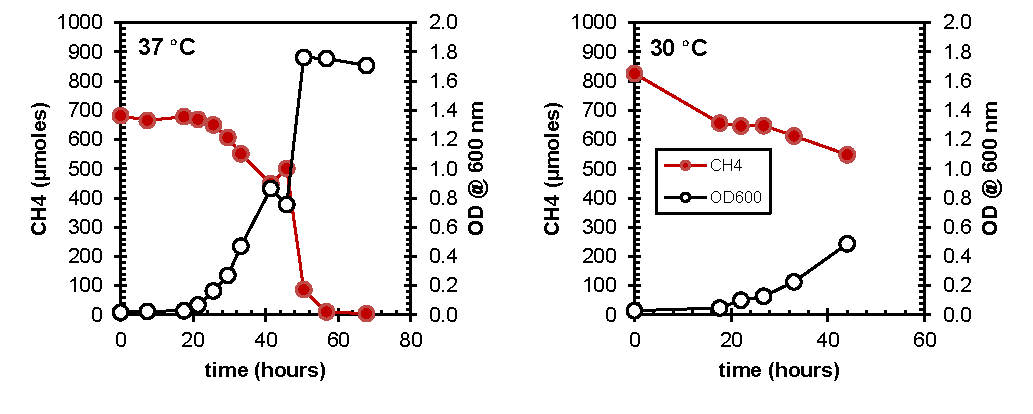
\includegraphics[width=0.95\textwidth]{figures/Fig4.S1}
	\caption[Preliminary growth curves of \emph{M. capsulatus} Bath]{Measured CH\textsubscript{4}
		concentrations and optical densities (OD) during preliminary experiments
		at 37~°C (left) and 30~°C (right) with starter cultures of \emph{M.}
		\emph{capsulatus} (Bath).}
	\label{fig:4:S1}
\end{figure*}

\emph{Methylococcus capsulatus} strain Bath cultures were grown in 10 ml
of nitrate mineral salts medium supplemented with 5~µM
CuSO\textsubscript{4} \parencite{Welander+Summons_2012_PNAS}. Serum bottles (160
cm\textsuperscript{3}) were inoculated with 2\%(v/v) inoculum from a
starter culture that had grown for ca.\ 30 hours, stoppered and sealed
without removing ambient air, and injected with 20 cm\textsuperscript{3}
SATP (\textasciitilde{}810~µmol) of methane from commercially-sourced
cylinders using a gas-tight syringe. Tests indicated that the starting
gas compositions were consistent within analytical error (±5\%) between
serum bottles. Multiple serum bottles were inoculated for each of the
two experimental temperatures (\autoref{tab:4:1}). Cultures were incubated at 30
or 37~°C while shaking at 225 rpm and sacrificed at given times by
adding 1 ml of 1 M hydrochloric acid. Each row in \autoref{tab:4:1} shows the
composition of one serum bottle at the time at which the experiment was
stopped. Experimental timepoints were selected based on monitoring of
growth during preliminary incubations of starter cultures (by tracking
optical density, see \autoref{fig:4:S1}). However, to minimize
puncturing of the serum bottles during the isotopic fractionation
experiments, optical densities were not measured for the samples
analyzed for isotopologues shown in \autoref{tab:4:1}. The combination of constant
agitation, a large headspace volume relative to liquid volume, and high
initial CH\textsubscript{4} partial pressures (\textgreater{}0.1 atm)
ensures that diffusion into the liquid from the headspace does not limit
the rate of methane consumption \parencite{Templeton++_2006_GCA,Nihous_2008_GCA}.

\subsection{Analytical techniques}\label{sec:4:analytical-techniques}

Concentrations of headspace gases, including CH\textsubscript{4} and
CO\textsubscript{2}, were determined via gas chromatography (GC) using a
Shimadzu GC-2014 gas chromatograph configured with a packed column
(Carboxen-1000, 5$'$ × 1/8$''$, Supelco, Bellefonte, Pennsylvania, USA) held
at 140~°C and argon carrier gas, and thermal conductivity and
methanizer-flame ionization detectors. Subsamples of the headspace (0.20
cm\textsuperscript{3} at laboratory temperature, \textasciitilde{}23~°C)
from each serum bottle were taken via a gas-tight syringe and injected
onto the column. Gas concentrations were determined directly as partial
pressures. Accuracy of the analyses, evaluated from standards, was ±5\%.
The fraction of initial methane remaining, \emph{f}, in each batch
culture was calculated from these measurements (\autoref{tab:4:1}), with
uncertainties propagated following \textcite{Ku_1969_JResNBS}.

Samples of methane were purified via cryofocusing--preparative gas
chromatography through a packed column (Carboxen-1000, 5$'$ × 1/8$''$,
Supelco) held at 30~°C with helium carrier gas, and cryotrapping of the
eluted methane on activated charcoal at liquid nitrogen temperature
\parencite{Wang++_2015_S}. The relative abundances of the methane stable
isotopologues \textsuperscript{12}CH\textsubscript{4},
\textsuperscript{13}CH\textsubscript{4},
\textsuperscript{12}CH\textsubscript{3}D, and
\textsuperscript{13}CH\textsubscript{3}D were measured using a tunable
infrared laser direct absorption spectroscopy technique described
previously \parencite{Ono++_2014_AC,Wang++_2015_S}.

Isotope values are reported herein using standard
delta-notation.\footnote{Definitions: δ\textsuperscript{13}C =
	(\textsuperscript{13}C/\textsuperscript{12}C)\textsubscript{sample}/(\textsuperscript{13}C/\textsuperscript{12}C)\textsubscript{PDB}
	$-$ 1, and δD = (D/H)\textsubscript{sample}/(D/H)\textsubscript{SMOW} $-$
	1 {[}for natural samples of methane, δ\textsuperscript{13}C~$\approx$~	(\textsuperscript{13}CH\textsubscript{4}/\textsuperscript{12}CH\textsubscript{4})\textsubscript{sample}/(\textsuperscript{13}CH\textsubscript{4}/\textsuperscript{12}CH\textsubscript{4})\textsubscript{PDB}
	$-$ 1 and δD $\approx$ ¼
	(\textsuperscript{12}CH\textsubscript{3}D/\textsuperscript{12}CH\textsubscript{4})\textsubscript{sample}/(D/H)\textsubscript{SMOW}
	$-$ 1{]}.} In accordance with IUPAC recommendations \parencite{Coplen_2011_RCM}, we
have omitted the factor of 1000‰ from the definition of δ and other
isotope values (including Δ\textsuperscript{13}CH\textsubscript{3}D,
below). Carbon and hydrogen isotope values were calibrated against
community reference materials NGS-1 and NGS-3 \parencite{Wang++_2015_S}.

The abundance of \textsuperscript{13}CH\textsubscript{3}D is tracked via
the Δ\textsuperscript{13}CH\textsubscript{3}D value, defined according
to \textcite{Ono++_2014_AC} as:
\begin{equation}\label{eqn:4:3}
\mathrm\Delta^{13}{\text{CH}}_3\text{D}=\ln Q\text{,\; where\ }Q=\frac{\bigl\lbrack{}^{13}{\text{CH}}_3\text{D}\bigr\rbrack\bigl\lbrack{}^{12}{\text{CH}}_4\bigr\rbrack}{\bigl\lbrack{}^{13}{\text{CH}}_4\bigr\rbrack\bigl\lbrack{}^{12}{\text{CH}}_3\text{D}\bigr\rbrack}
\end{equation}
Here, \emph{Q} is the reaction quotient for \mrefs[]{Reaction}{eqn:4:2}, and
Δ\textsuperscript{13}CH\textsubscript{3}D $ \approx $ \emph{Q} $-$ 1 because
\emph{Q} is close to unity in the natural and experimental systems
studied herein.\footnote{From the approximation
	\(\ln{\left( 1 + x \right) \approx x}\) for values of \emph{x} close
	to zero.} For a methane sample that has attained a distribution of
isotopes among all isotopologues consistent with equilibrium at a given
temperature, \emph{Q} = \emph{K}. The temperature dependence of the
equilibrium Δ\textsuperscript{13}CH\textsubscript{3}D value was
theoretically estimated and experimentally calibrated previously \parencite{Wang++_2015_S}.

Methane samples with a wide range of δD values ($-$480‰ to +500‰ vs.\ SMOW) were prepared and thermally-equilibrated over platinum catalyst at
300~°C to correct for the nonlinearity in the spectroscopic analysis
described by \textcite{Ono++_2014_AC}.

\subsection{Calculation of isotope and isotopologue fractionation
	factors}\label{sec:4:calculation-of-isotope-and-isotopologue-fractionation-factors}

The MMO-catalyzed reaction between methane and O\textsubscript{2} to
produce the intermediate product methanol is the first in a sequence of
enzymatic reactions involved in aerobic methanotrophy \parencite{Sirajuddin+Rosenzweig_2015_Bc}. We focus on this reaction because it is the most
important isotopically-fractionating step in this sequence as it is
considered to be both rate-limiting and isotope-sensitive \parencite{Nesheim+Lipscomb_1996_Bc} under the studied experimental conditions. Limitation of
the rate of methane consumption by this step requires that methane
diffusion into and out of the cells be rapid relative to MMO catalysis.
Following \textcite{Nihous_2010_IEHS}, we assume that isotopic fractionation
associated with transfer of methane across cell membranes is negligible.

The reaction scheme for the first step of the aerobic oxidation of the
methane isotopologues \textsuperscript{12}CH\textsubscript{4},
\textsuperscript{13}CH\textsubscript{4},
\textsuperscript{12}CH\textsubscript{3}D, and
\textsuperscript{13}CH\textsubscript{3}D can be described by the
following six chemical reactions:
\begin{align}
{}^{12}{\text{CH}}_4&\longrightarrow{}^{12}{\text{CH}}_3\text{OH} \label{eqn:4:4}\\
{}^{13}{\text{CH}}_4&\longrightarrow{}^{13}{\text{CH}}_3\text{OH} \label{eqn:4:5}\\
{}^{12}{\text{CH}}_3\text{D}&\longrightarrow{}^{12}{\text{CH}}_3\text{OH} \label{eqn:4:6}\\
{}^{12}{\text{CH}}_3\text{D}&\longrightarrow{}^{12}{\text{CH}}_2\text{DOH} \label{eqn:4:7}\\
{}^{13}{\text{CH}}_3\text{D}&\longrightarrow{}^{13}{\text{CH}}_3\text{OH} \label{eqn:4:8}\\
{}^{13}{\text{CH}}_3\text{D}&\longrightarrow{}^{13}{\text{CH}}_2\text{DOH} \label{eqn:4:9}
\end{align}

\subsubsection{Carbon isotope
	fractionation}\label{sec:4:carbon-isotope-fractionation}

Assuming that the reaction is irreversible, follows first-order
kinetics, and occurs in a closed system, the following differential
equations can be written for \textsuperscript{12}CH\textsubscript{4} and
\textsuperscript{13}CH\textsubscript{4}:
\begin{align}
\frac{d_{}^{\mathrm{12}}{\mathrm{C}\mathrm{H}_{\mathrm{4}}}}{{dt}} &= - k \cdot \bigl\lbrack{}_{}^{\mathrm{12}}{\mathrm{C}\mathrm{H}_{\mathrm{4}}} \bigr\rbrack \label{eqn:4:10} \\
\frac{d_{}^{\mathrm{13}}{\mathrm{C}\mathrm{H}_{\mathrm{4}}}}{{dt}} &= -_{}^{13}\alpha \cdot k \cdot \bigl\lbrack{}_{}^{\mathrm{13}}{\mathrm{C}\mathrm{H}_{\mathrm{4}}} \bigr\rbrack \label{eqn:4:11}
\end{align}
where \emph{k} is the rate constant for
\textsuperscript{12}CH\textsubscript{4} consumption (\mrefs[]{Reaction}{eqn:4:4}), and
\textsuperscript{13}$\alpha$ is the fractionation factor for
\textsuperscript{13}C/\textsuperscript{12}C (ratio of rate constants for
\mrefs[]{Reactions}{eqn:4:5} and \ref{eqn:4:4}).

Combining \mrefs[]{Eqns.}{eqn:4:10} and \ref{eqn:4:11}, eliminating \emph{dt}, and integrating from
\emph{f} = 1 (initial) to \emph{f} yields the equation:
\begin{equation}\label{eqn:4:12}
\ln\left( \frac{\bigl\lbrack{}_{}^{\mathrm{13}}{\mathrm{C}\mathrm{H}_{\mathrm{4}}} \bigr\rbrack_{f}}{\bigl\lbrack{}_{}^{\mathrm{13}}{\mathrm{C}\mathrm{H}_{\mathrm{4}}} \bigr\rbrack_{\mathrm{\text{init}}}} \right) = {}_{}^{13}\alpha \cdot \ln\left( \frac{\bigl\lbrack{}_{}^{\mathrm{12}}{\mathrm{C}\mathrm{H}_{\mathrm{4}}} \bigr\rbrack_{f}}{\bigl\lbrack{}_{}^{\mathrm{12}}{\mathrm{C}\mathrm{H}_{\mathrm{4}}} \bigr\rbrack_{\mathrm{\text{init}}}} \right)
\end{equation}

By subtracting
\(\ln\left( {\bigl\lbrack{}_{}^{\mathrm{12}}{\mathrm{C}\mathrm{H}_{\mathrm{4}}} \bigr\rbrack_{f}}\middle/{\bigl\lbrack{}_{}^{\mathrm{12}}{\mathrm{C}\mathrm{H}_{\mathrm{4}}} \bigr\rbrack_{\mathrm{\text{init}}}} \right)\)
from each side of \autoref{eqn:4:12}, and applying the approximations
\(f \approx \allowbreak \left.{\bigl\lbrack{}_{}^{\mathrm{12}}{\mathrm{C}\mathrm{H}_{\mathrm{4}}} \bigr\rbrack_{f}}\middle/{\bigl\lbrack{}_{}^{\mathrm{12}}{\mathrm{C}\mathrm{H}_{\mathrm{4}}} \bigr\rbrack_{\mathrm{\text{init}}}}\right.\)
and
{[}\textsuperscript{13}CH\textsubscript{4}{]}$\big/${[}\textsuperscript{12}CH\textsubscript{4}{]}
$ \approx $ {[}\textsuperscript{13}C{]}$\big/${[}\textsuperscript{12}C{]}, we obtain a form of the
classic ``Rayleigh equation'' \parencite{Mariotti++_1981}:
\begin{equation}\label{eqn:4:13}
\ln\frac{\mathrm{\updelta}^{13}\mathrm{C} + 1}{{\mathrm{\updelta}^{13}\mathrm{C}}_{\mathrm{\text{init}}} + 1} = \left({}_{}^{13}\alpha - 1 \right)\,\ln f
\end{equation}

\subsubsection{Hydrogen isotope
	fractionation}\label{sec:4:hydrogen-isotope-fractionation}

For the D-substituted isotopologue
\textsuperscript{12}CH\textsubscript{3}D, there are two ways to break a
carbon-hydrogen bond. These two pathways are described by \mrefs[]{Reactions}{eqn:4:6} and \ref{eqn:4:7}. The former involves the breakage of the C--D bond (accompanied by
a primary isotope effect, described by the fractionation factor
\textsuperscript{D}$\alpha$\textsubscript{p}), while the latter involves the
breakage of any of the three C--H bonds \emph{adjacent} to the C--D bond
(incurring a secondary isotope effect,
\textsuperscript{D}$\alpha$\textsubscript{s}). Thus, the overall rate of the
oxidation of \textsuperscript{12}CH\textsubscript{3}D to methanol can be
described by:
\begin{equation}\label{eqn:4:14} 
\frac{d_{}^{\mathrm{12}}{\mathrm{C}\mathrm{H}_{\mathrm{3}}\mathrm{D}}}{{dt}} = \textstyle - \frac{1}{4} \cdot{}_{}^{\mathrm{D}}\alpha_{\mathrm{p}} \cdot k \cdot \bigl\lbrack{}_{}^{\mathrm{12}}{\mathrm{C}\mathrm{H}_{\mathrm{3}}\mathrm{D}} \bigr\rbrack - \frac{3}{4} \cdot{}_{}^{\mathrm{D}}\alpha_{\mathrm{s}} \cdot k \cdot \bigl\lbrack{}_{}^{\mathrm{12}}{\mathrm{C}\mathrm{H}_{\mathrm{3}}\mathrm{D}} \bigr\rbrack
\end{equation}

By lumping together \textsuperscript{D}$\alpha$\textsubscript{p} and
\textsuperscript{D}$\alpha$\textsubscript{s}, the rate equation can be
simplified to:
\begin{equation}\label{eqn:4:15}
\frac{d_{}^{\mathrm{12}}{\mathrm{C}\mathrm{H}_{\mathrm{3}}\mathrm{D}}}{{dt}} = \textstyle -_{}^{\mathrm{D}}\alpha \cdot k \cdot \bigl\lbrack{}_{}^{\mathrm{12}}{\mathrm{C}\mathrm{H}_{\mathrm{3}}\mathrm{D}} \bigr\rbrack
\end{equation}
where
\(_{}^{\mathrm{D}}\alpha = \frac{1}{4}{}_{}^{\mathrm{D}}\alpha_{\mathrm{p}} + \frac{3}{4}{}_{}^{\mathrm{D}}\alpha_{\mathrm{s}}\).

This parameterization of D/H fractionation is attractive in that it
allows for apparent overall isotopic fractionation factors to be
constrained by cell culture experiments and measurement with
conventional geochemical techniques (e.g., isotope ratio mass
spectrometry), without measurement of the individual reaction products.
Applying the same logic used in \autoref{sec:4:carbon-isotope-fractionation}, the following expression is
obtained:
\begin{equation}\label{eqn:4:16}
\ln\frac{\mathrm{\text{δD}} + 1}{\mathrm{\text{δD}}_{\mathrm{\text{init}}} + 1} = \left(_{}^{\mathrm{D}}\alpha - 1 \right)\,\ln f
\end{equation}

Combining \mrefs{Eqns.}{eqn:4:13} and~\ref{eqn:4:16} yields an equation describing the correlation
between carbon and hydrogen isotope fractionation:

\begin{equation}\label{eqn:4:17}
\ln\frac{\mathrm{\text{δD}} + 1}{\mathrm{\text{δD}}_{\mathrm{\text{init}}} + 1} = \left( \frac{{}_{}^{\mathrm{D}}\alpha - 1}{{}_{}^{13}\alpha - 1} \right)\ln\frac{\mathrm{\updelta}^{13}\mathrm{C} + 1}{{\mathrm{\updelta}^{13}\mathrm{C}}_{\mathrm{\text{init}}} + 1}
\end{equation}

\subsubsection{\texorpdfstring{\textsuperscript{13}CH\textsubscript{3}D
		fractionation}{13CH3D fractionation}}\label{sec:4:13ch3d-fractionation}

The rate of oxidation of \textsuperscript{13}CH\textsubscript{3}D can be
described by:
\begin{equation}\label{eqn:4:18}
\frac{d_{}^{\mathrm{13}}{\mathrm{C}\mathrm{H}_{\mathrm{3}}\mathrm{D}}}{{dt}} = \textstyle - \frac{1}{4} \cdot \gamma_{\mathrm{p}} \cdot{}_{}^{13}\alpha \cdot{}_{}^{\mathrm{D}}\alpha_{\mathrm{p}} \cdot k \cdot \bigl\lbrack{}_{}^{\mathrm{13}}{\mathrm{C}\mathrm{H}_{\mathrm{3}}\mathrm{D}} \bigr\rbrack - \frac{3}{4} \cdot \gamma_{\mathrm{s}} \cdot{}_{}^{13}\alpha \cdot{}_{}^{\mathrm{D}}\alpha_{\mathrm{s}} \cdot k \cdot \bigl\lbrack{}_{}^{\mathrm{13}}{\mathrm{C}\mathrm{H}_{\mathrm{3}}\mathrm{D}} \bigr\rbrack
\end{equation}

Here, we have introduced the terms $\gamma$\textsubscript{p} and
$\gamma$\textsubscript{s} to characterize deviations of the clumped
isotopologue fractionation factor from the product of the
\textsuperscript{13}C/\textsuperscript{12}C and D/H fractionation
factors ($\alpha$ values). When there is no deviation from this product (i.e.,
primary and secondary isotope fractionation factors for bond breakage in
\textsuperscript{13}CH\textsubscript{3}D follow what is referred to
hereafter as the ``product rule''), both $\gamma$\textsubscript{p} and
$\gamma$\textsubscript{s} are unity. Deviations from the product rule represent
a ``clumped isotopologue effect'' on bond breakage that arises from the
substitution of both \textsuperscript{13}C and D in the substrate
methane. To simplify the treatment of clumped isotopologue effects in
the absence of literature data for $\gamma$\textsubscript{p} and
$\gamma$\textsubscript{s}, we adopt the following form of the rate equation:
\begin{equation}\label{eqn:4:19}
\frac{d_{}^{\mathrm{13}}{\mathrm{C}\mathrm{H}_{\mathrm{3}}\mathrm{D}}}{{dt}} = - \gamma \cdot{}_{}^{13}\alpha \cdot{}_{}^{\mathrm{D}}\alpha \cdot k \cdot \bigl\lbrack{}_{}^{\mathrm{13}}{\mathrm{C}\mathrm{H}_{\mathrm{3}}\mathrm{D}} \bigr\rbrack
\end{equation}

Here, the ``gamma-factor'' ($\gamma$) is an empirically-constrained term that
describes an \emph{effective} clumped isotopologue fractionation factor.
Implicit in the use of \autoref{eqn:4:19} is that
\(\gamma \cdot{}_{}^{\mathrm{D}}\alpha = \frac{1}{4} \cdot \gamma_{\mathrm{p}} \cdot{}_{}^{\mathrm{D}}\alpha_{\mathrm{p}} + \frac{3}{4} \cdot \gamma_{\mathrm{s}} \cdot{}_{}^{\mathrm{D}}\alpha_{\mathrm{s}}\)
(from the definition of \textsuperscript{D}$\alpha$ in \autoref{sec:4:hydrogen-isotope-fractionation}; also see
discussion in \autoref{sec:4:fractionation-of-13ch3d}). This condition is satisfied, although not
uniquely, when $\gamma$ is equal to both $\gamma$\textsubscript{p} and
$\gamma$\textsubscript{s}.

\mrefs[]{Equation}{eqn:4:19} is convenient because it allows for $\gamma$ to be constrained by
measurements of the methane isotopologues in experiments conducted at
natural abundance without the use of isotopically labeled substrates or
measurement of individual isotopically-substituted products. Integration
of \autoref{eqn:4:19} combined with \autoref{eqn:4:10}, subtraction of the isotopologue-ratio
forms of \mrefs[]{Eqns.}{eqn:4:13} and \autoref{eqn:4:16} from the result, and substitution of the
definition of Δ\textsuperscript{13}CH\textsubscript{3}D (\autoref{eqn:4:3}) yields:
\begin{equation}\label{eqn:4:20}
\Delta_{}^{\mathrm{13}}{\mathrm{C}\mathrm{H}_{\mathrm{3}}\mathrm{D}} = {\Delta_{}^{\mathrm{13}}{\mathrm{C}\mathrm{H}_{\mathrm{3}}\mathrm{D}}}_{\mathrm{\text{initial}}} + \left( \gamma \cdot{}_{}^{13}\alpha \cdot{}_{}^{\mathrm{D}}\alpha -{}_{}^{13}\alpha -{}_{}^{\mathrm{D}}\alpha + 1 \right) \cdot \ln f\
\end{equation}

Adopting this greatly simplified treatment necessarily means that
differences in primary and secondary isotope effects for different forms
of the enzyme in different methanotroph species are masked and lumped
into an ``effective'' fractionation factor. A similar line of reasoning
was used by \textcite{Stolper++_2015_GCA} to simplify the representation of a
model methanogenic system.

\section{Results }\label{sec:4:results}


\begin{SCfigure}
	\centering
	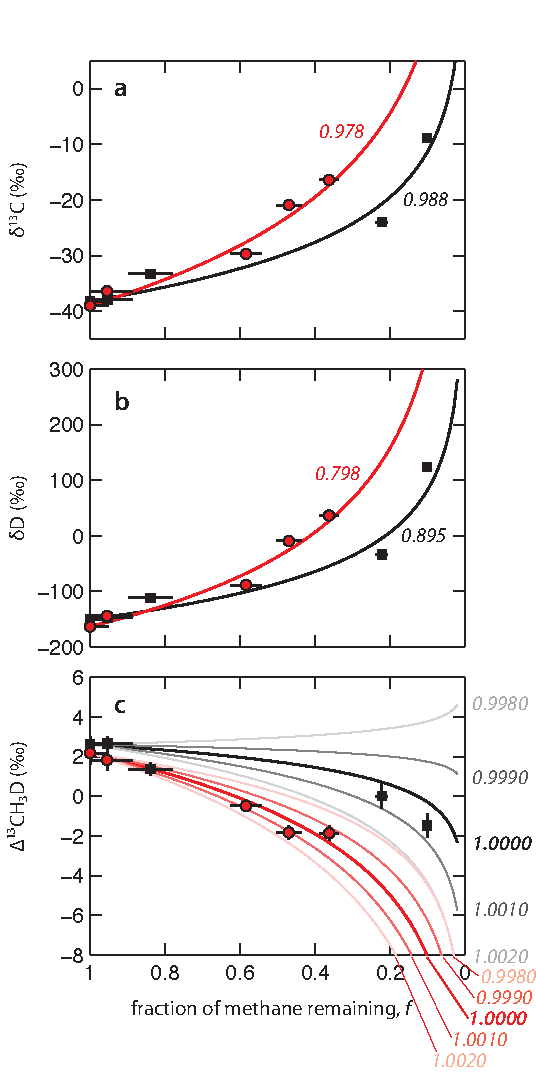
\includegraphics[width=0.5\textwidth]{figures/Fig4.1}
	\caption[Measured and modeled δ\textsuperscript{13}C, δD, and Δ\textsuperscript{13}CH\textsubscript{3}D values in batch cultures]{Measured and modeled changes in \textbf{(a)}
		δ\textsuperscript{13}C, \textbf{(b)} δD, and \textbf{(c)}
		Δ\textsuperscript{13}CH\textsubscript{3}D of residual methane as a
		function of \emph{f}, the fraction of initial methane remaining. Data
		points from the 30 and 37~°C experiments (\autoref{tab:4:1}) are shown with black
		and red symbols, respectively. Horizontal error bars represent
		propagated ±1$\sigma$ uncertainties from GC measurements, and vertical error
		bars represent 95\% confidence intervals from isotopologue ratio
		analyses. Solid lines represent the modeled values (from \mrefs[]{Eqns.}{eqn:4:13}, \ref{eqn:4:16},
		and \ref{eqn:4:20}) based on the calculated weighted-average carbon- and
		hydrogen-isotope fractionation factors for each set of experiments as
		listed in \autoref{tab:4:1}. Labels in \emph{italics} represent
		\textsuperscript{13}$\alpha$, \textsuperscript{D}$\alpha$, \& $\gamma$, respectively, in
		panels (a), (b), \& (c). Panel (c) shows model results calculated
		assuming different values of $\gamma$ varying between 0.9980 and 1.0020.}
	\label{fig:4:1}
\end{SCfigure}


\begin{sidewaystable}\centering
	\begin{threeparttable}
		\caption[Experimental results and calculated fractionation
		factors for batch cultures of \emph{M.\ capsulatus}]{Experimental results and calculated fractionation
		factors for batch cultures of \emph{Methylococcus capsulatus} Bath.
		Uncertainties (±1$\sigma$) listed for \emph{f}, \textsuperscript{13}$\alpha$,
		\textsuperscript{D}$\alpha$, and $\gamma$ are propagated from those associated with
		individual measurements according to standard formulas \parencite{Ku_1969_JResNBS}.}
		\label{tab:4:1}
		\begin{tabular}{lc r@{\;}c@{\;}l r r r r@{\;}c@{\;}l r@{\;}c@{\;}l r@{\;}c@{\;}l r@{\;}c@{\;}l}
			\toprule
			& time (h) & \multicolumn{3}{c}{\emph{f}} & CO\textsubscript{2}
			(cm\textsuperscript{3})\tnote{a} & δ\textsuperscript{13}C
			(‰)\tnote{c} & δD (‰)\tnote{c} & \multicolumn{3}{c}{
			Δ\textsuperscript{13}CH\textsubscript{3}D (‰)\tnote{c} } &
			\multicolumn{3}{c}{ \textsuperscript{13}$\alpha$ } & \multicolumn{3}{c}{ \textsuperscript{D}$\alpha$ } & \multicolumn{3}{c}{ $\gamma$ }\tabularnewline
			\midrule
			& & & & & & & & & & & & & & & & & & &\tabularnewline
			\emph{30~°C} & 0 & 1.00 & ± & 0.05\tnote{b} & \textless{}0.2 &
			$-$38.27 & $-$150.12 & 2.61 & ± & 0.43 & & & & & & & & &\tabularnewline
			& 12 & 0.95 & ± & 0.07 & 0.6 & $-$37.94 & $-$147.20 & 2.66 & ± & 0.34 &
			0.993 & ± & 0.011 & 0.928 & ± & 0.107 & 0.9983 & ± &
			0.0130\tabularnewline
			& 36 & 0.84 & ± & 0.06 & 1.9 & $-$33.31 & $-$111.79 & 1.36 & ± & 0.34 &
			0.971 & ± & 0.012 & 0.749 & ± & 0.101 & 0.9997 & ± &
			0.0060\tabularnewline
			& --\tnote{d} & 0.22 & ± & 0.02 & 10.3 & $-$24.00 & $-$33.36 &
			$-$0.01 & ± & 0.60 & 0.990 & ± & 0.0005 & 0.915 & ± & 0.004 & 1.0010 & ± &
			0.0005\tabularnewline
			& 60 & 0.10 & ± & 0.01 & 9.8 & $-$8.81 & 123.90 & $-$1.48 & ± & 0.60 & 0.987
			& ± & 0.0004 & 0.878 & ± & 0.004 & 1.0002 & ± & 0.0004\tabularnewline \cmidrule{12-20} 
			& & & & & & & \multicolumn{4}{r}{weighted average\tnote{e}} & 0.988 & ± & 0.0003 &
			0.895 & ± & 0.003 & 1.0005 & ± & 0.0003\tabularnewline
			& & & & & & & & & & & & & & & & & & &\tabularnewline
			\emph{37~°C} & 0 & 1.00 & ± & 0.05\tnote{b} & n.d. & $-$39.06 &
			$-$163.57 & 2.17 & ± & 0.59 & & & & & & & & &\tabularnewline
			& 41 & 0.95 & ± & 0.07 & n.d. & $-$36.45 & $-$144.23 & 1.82 & ± & 0.53 &
			0.943 & ± & 0.086 & 0.516 & ± & 0.726 & 0.9585 & ± &
			0.2130\tabularnewline
			& 44 & 0.58 & ± & 0.04 & 2.5 & $-$29.68 & $-$88.51 & $-$0.48 & ± & 0.30 &
			0.982 & ± & 0.002 & 0.840 & ± & 0.021 & 1.0025 & ± &
			0.0015\tabularnewline
			& 48 & 0.47 & ± & 0.03 & 4.8 & $-$20.95 & $-$9.20 & $-$1.82 & ± & 0.36 & 0.975
			& ± & 0.002 & 0.776 & ± & 0.021 & 0.9997 & ± & 0.0014\tabularnewline
			& 51 & 0.36 & ± & 0.03 & 6.3 & $-$16.39 & 36.83 & $-$1.87 & ± & 0.38 & 0.977
			& ± & 0.002 & 0.788 & ± & 0.015 & 0.9989 & ± & 0.0011\tabularnewline \cmidrule{12-20} 
			& & & & & & & \multicolumn{4}{r}{weighted average\tnote{e}} & 0.978 & ± & 0.001 &
			0.798 & ± & 0.010 & 1.0000 & ± & 0.0007\tabularnewline
			& & & & & & & & & & & & & & & & & & &\tabularnewline
			\bottomrule
		\end{tabular}
		{\small n.d., not determined}
		\begin{tablenotes}
				\item[a] Total inorganic carbon in the bottle (including
				gaseous CO\textsubscript{2} and dissolved inorganic carbon), reported as
				cm\textsuperscript{3}-equivalent of CO\textsubscript{2} at standard
				ambient temperature and pressure (SATP; 25~°C, 1 bar), was estimated
				from headspace CO\textsubscript{2} concentration (determined via GC),
				the Henry's law constant for CO\textsubscript{2} at room temperature,
				and the volume of headspace and of HCl-spiked medium. Uncertainty is
				estimated at ±10\%. Quantitative conversion of initial
				CH\textsubscript{4} (see \autoref{sec:4:cultures}) into CO\textsubscript{2} (i.e., 100\%
				oxidation with no incorporation of CH\textsubscript{4}-derived carbon
				into biomass) would yield 20~cm\textsuperscript{3} SATP of
				CO\textsubscript{2}.
				
				\item[b] An uncertainty of ±5\% was assigned to the initial
				value of \emph{f} to account for variability in starting amounts of
				methane between bottles (see \autoref{sec:4:cultures}). This uncertainty is propagated
				throughout the calculations for later timepoints.
				
				\item[c] Values for δ\textsuperscript{13}C, δD, and
				Δ\textsuperscript{13}CH\textsubscript{3}D are reported relative to PDB,
				SMOW, and the stochastic distribution, respectively. Uncertainties for
				δ\textsuperscript{13}C, δD (both ca.\ 0.1‰), and
				Δ\textsuperscript{13}CH\textsubscript{3}D (listed) are 95\% confidence
				intervals over all cycles in a single analysis \parencite[e.g.,][]{Wang++_2015_S},
				but are conservatively treated as 1$\sigma$ for purposes of error propagation.
				
				\item[d] Time not recorded.
				
				\item[e] Weighted means of each set of \textsuperscript{13}$\alpha$,
				\textsuperscript{D}$\alpha$, and $\gamma$ values, weighted by 1/$\sigma$\textsuperscript{2}.
				Uncertainty (1$\sigma$) in weighted means was estimated following \textcite{Bevington+Robinson_3e}.
		\end{tablenotes}
	\end{threeparttable}
\end{sidewaystable}


During the course of the experiments at 30 and 37~°C, the concentration
of methane in the headspace decreased and the concentration of
CO\textsubscript{2} increased (\autoref{tab:4:1}). The bottles incubated at 37~°C
exhibited a lag phase (observed in preliminary experiments with starter
cultures, \autoref{fig:4:S1}), with a rapid transition into active
methane consumption around 41 hours after inoculation (\autoref{tab:4:1}), whereas
in the 30~°C experiments, methane consumption began immediately after
inoculation, but at an apparently lower rate. Based on mass balance of
measured CO\textsubscript{2} and CH\textsubscript{4} concentrations
relative to initial CH\textsubscript{4} (\autoref{tab:4:1}), \textasciitilde{}7\%
to 41\% of carbon was not accounted for; this fraction of carbon was
likely incorporated into cellular biomass (\emph{b} in \autoref{eqn:4:1}). This
range of \emph{b} values is similar to ranges observed in previous
studies \parencite[e.g., 0.1$-$0.5 in][]{Templeton++_2006_GCA}.

The initial isotopic composition of the methane used was different
between the two sets of experiments (\autoref{tab:4:1}). As methane was consumed,
the δ\textsuperscript{13}C and δD values of the residual methane
increased (\autoref{fig:4:1}), indicating a preferential consumption of the lighter
\textsuperscript{12}C and \textsuperscript{1}H by the bacteria.
Conversely, Δ\textsuperscript{13}CH\textsubscript{3}D values of the
residual methane decreased as methane was consumed, starting from
initial values of ca.\ +2.6‰ and +2.2‰, and decreasing to ``anticlumped''
(\textless{}0‰) values of ca.\ $-$1.5‰ and $-$1.9‰, respectively, at the last
time points sampled in the 30 and 37~°C experiments (\autoref{tab:4:1}).

Using \mrefs{Eqns.}{eqn:4:13}, \ref{eqn:4:16}, and \ref{eqn:4:20}, values of the fractionation factors
\textsuperscript{13}$\alpha$, \textsuperscript{D}$\alpha$, and $\gamma$ were calculated for
each time point after the initial (\autoref{tab:4:1}). All calculations used the
initial timepoint as the reference starting point; thus, the
fractionation factors reported are averaged over the entire reaction
occurring in the bottle, and contain correlated errors linked to the
uncertainty in data from the initial timepoint. Fractionation factors
were calculated for each timepoint, rather than over all bottles in an
experiment, to avoid artifacts from variable growth between bottles,
particularly at the lower temperature of 30~°C (see \autoref{fig:4:S1}). In the earlier time points, the error in the calculated
fractionation factors is large because of uncertainties in \emph{f} and
in Δ\textsuperscript{13}CH\textsubscript{3}D. For each set of
experiments, the weighted-averages of the fractionation factors were
determined, and are listed in \autoref{tab:4:1}, and the corresponding
trajectories (using experimental \textsuperscript{13}$\alpha$ and
\textsuperscript{D}$\alpha$ values, and variable $\gamma$) are depicted in \autoref{fig:4:1}.

Isotopic fractionation of D/H was substantially greater in magnitude
than that of \textsuperscript{13}C/\textsuperscript{12}C (\mrefs[a]{Fig.}{fig:4:2}). In
general, a greater degree of both carbon- and hydrogen-isotope
fractionation was observed in the bottles incubated at 37~°C than at 30
°C (\mrefs[b]{Fig.}{fig:4:2}). No systematic changes in the magnitude of isotope
fractionation were observed over the course of the experiments (\autoref{tab:4:1}). A similar, tight correlation of D/H and
\textsuperscript{13}C/\textsuperscript{12}C fractionation is observed
between the two sets of experiments (\mrefs[a]{Fig.}{fig:4:2}).

Calculated $\gamma$ values for each experimental timepoint are shown in \autoref{tab:4:1}. All values were close to unity, and showed no systematic changes over
the course of incubation. The weighted-average $\gamma$ values for the
experiments were identical to unity within 2$\sigma$ error (1.0005 ± 0.0006 and
1.0000 ± 0.0014 for the 30 and 37~°C experiments, respectively).

\section{Discussion}\label{sec:4:discussion}

\subsection{Isotope and isotopologue fractionation during aerobic
	methanotrophy}\label{sec:4:isotope-and-isotopologue-fractionation-during-aerobic-methanotrophy}

\subsubsection{\texorpdfstring{Fractionation of methane
		\textsuperscript{13}C/\textsuperscript{12}C and D/H
		ratios}{Fractionation of methane 13C/12C and D/H ratios}}\label{sec:4:fractionation-of-methane-13c12c-and-dh-ratios}

A wide range of carbon isotope fractionation factors
{[}\textsuperscript{13}$\varepsilon$ (= \textsuperscript{13}$\alpha$ $-$ 1) ranging from $-$38‰
to $-$3‰{]} have been reported in culture- and field-based studies \parencite[see][and references therein]{Templeton++_2006_GCA}. The variable nature
of the magnitude of observed carbon isotope effects complicates
application of measurements of individual carbon isotope ratios in
diagnosing the presence and extent of methanotrophy in the environment.
As such, the use of paired δ\textsuperscript{13}C and δD data has been
suggested as a possible method of removing some levels of ambiguity
associated with the sole use of carbon isotopes \parencite{Elsner++_2005_EST}.
Although the absolute magnitudes of isotope fractionation may vary due
to ``masking effects'' from preceding isotopically-insensitive steps
such as transport across membranes or binding to an enzyme \parencite{Feisthauer++_2011_GCA}, a correlation between the fractionation of the carbon and
hydrogen isotopes can be expected because both are principally
influenced by the breakage of the C--H bond. Such a correlation was
first noted by \textcite{Coleman++_1981_GCA}, with later studies by \textcite{Kinnaman++_2007_GCA,Powelson++_2007_EST,Feisthauer++_2011_GCA} corroborating
the observations in pure culture and in enrichments from other
environments. The published values of
\textsuperscript{D}$\varepsilon$/\textsuperscript{13}$\varepsilon$, corresponding to the slope
of the gray lines in \mrefs[a]{Fig.}{fig:4:2}, range from 5.9 to 14.9, with a mean of 8.9
± 2.3 {[}standard deviation (1$\sigma$), \emph{n} = 15{]}. The best-fit value
of \textsuperscript{D}$\varepsilon$/\textsuperscript{13}$\varepsilon$ for the data shown in
\autoref{tab:4:1} is 9.14, a value which appears independent of the two growth
temperatures tested, and which falls near the middle of the published
range.


\begin{figure*}
	\centering
	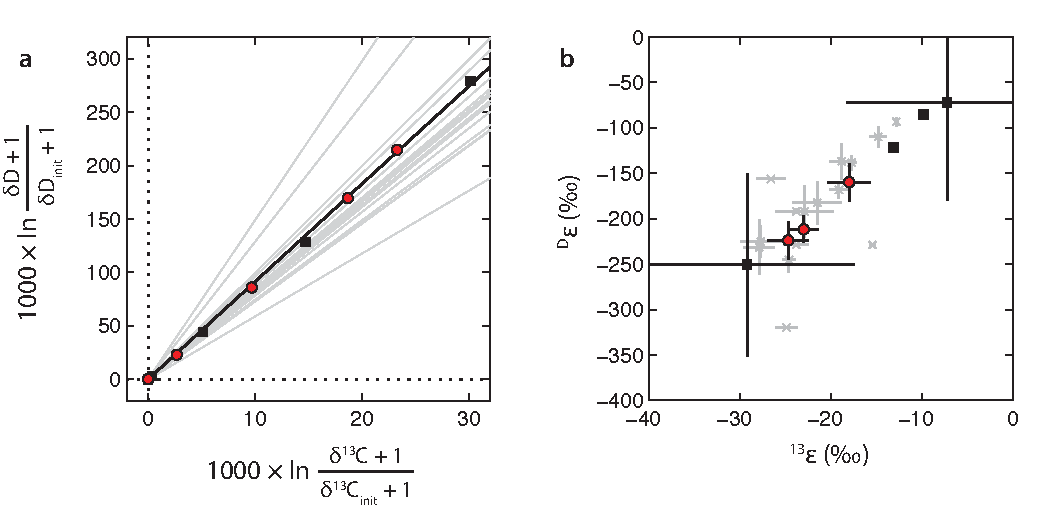
\includegraphics[width=0.95\textwidth]{figures/Fig4.2}
	\caption[\textsuperscript{13}C/\textsuperscript{12}C and D/H fractionation by aerobic methanotrophs]{Relationship between fractionation of carbon and
		hydrogen isotopes. \textbf{(a)} Data from the 30 and 37~°C experiments (\autoref{tab:4:1})
		are shown with black and red symbols, respectively. Black line (\emph{y}
		= 9.14 \emph{x}) represents the best-fit regression through the data.
		From \autoref{eqn:4:17}, the slope of this line is (\textsuperscript{D}$\alpha$ $-$
		1)/(\textsuperscript{13}$\alpha$ $-$ 1), or
		\textsuperscript{D}$\varepsilon$/\textsuperscript{13}$\varepsilon$. Near the origin, the
		\emph{x}- and \emph{y}-axes are approximately equal to
		δ\textsuperscript{13}C $-$ δ\textsuperscript{13}C\textsubscript{init} and
		δD $-$ δD\textsubscript{init}, respectively; this approximation becomes
		less accurate with increasing distance from the origin, particularly for
		hydrogen \parencite{Sessions+Hayes_2005_GCA}. Gray lines represent
		previously-reported correlations between fractionation of carbon and
		hydrogen isotopes by aerobic methanotrophs determined from experiments
		with pure cultures \parencite{Feisthauer++_2011_GCA} and enrichment cultures
		\parencite{Coleman++_1981_GCA,Kinnaman++_2007_GCA,Powelson++_2007_EST}.
		\textbf{(b)} Fractionation factors ($\varepsilon$, defined as $\alpha$ $-$ 1) calculated for
		individual bottle incubations from this study (\autoref{tab:4:1}) plotted against
		fractionation factors reported in the cited studies (gray). One point
		from the 37~°C experiment (41 h) was not plotted because of large
		uncertainties arising from a minimal extent of reaction.}
	\label{fig:4:2}
\end{figure*}


The consistency of the determined
\textsuperscript{D}$\varepsilon$/\textsuperscript{13}$\varepsilon$ ratios with those in the
literature provides confidence that results regarding the behavior of
Δ\textsuperscript{13}CH\textsubscript{3}D (discussed below) during
aerobic methane oxidation by \emph{M.~capsulatus} (Bath) can be
generalizable to other strains grown under other conditions. Further
experiments with these strains grown under different conditions to
examine clumped isotopologue fractionation will help to determine if
this hypothesis is valid. In a previous study, various strains of
bacteria \parencite[including \emph{M.~capsulatus}, which has two pMMOs and one
sMMO;][]{Ward++_2004_PLOSBiol} grown in batch cultures under different
copper (Cu) concentrations (with pMMO expressed under Cu-rich conditions
and sMMO under low Cu) demonstrated consistently correlated
fractionations of carbon and hydrogen isotopes, without apparent
correlation to physiology or growth condition \parencite{Feisthauer++_2011_GCA}.
Values of \textsuperscript{D}$\varepsilon$/\textsuperscript{13}$\varepsilon$ derived from that
study range from 7.3 to 8.8, and are close to the average
\textsuperscript{D}$\varepsilon$/\textsuperscript{13}$\varepsilon$ ratio from our dataset (9.14, \mrefs[a]{Fig.}{fig:4:2}). In particular, \emph{M.~cap\-su\-la\-tus} grown at 45~°C induced
isotopic fractionations of \textsuperscript{13}$\alpha$ = 0.972 ± 0.002 and
\textsuperscript{D}$\alpha$ = 0.769 ± 0.030 (published uncertainties were
listed as 95\% confidence interval, approximately 2$\sigma$) under Cu-rich
conditions, and under Cu-poor conditions, similar values of
\textsuperscript{13}$\alpha$ = 0.977 ± 0.003 and \textsuperscript{D}$\alpha$ = 0.808 ±
0.029 \parencite{Feisthauer++_2011_GCA}. The corresponding
\textsuperscript{D}$\varepsilon$/\textsuperscript{13}$\varepsilon$ ratios (with propagated
\textasciitilde{}2$\sigma$ uncertainties) indicated by their data are 8.3 ± 1.1
and 8.4 ± 1.7 under Cu-rich and Cu-poor conditions, respectively. These
values are indistinguishable from the
\textsuperscript{D}$\varepsilon$/\textsuperscript{13}$\varepsilon$ ratio derived from regression
through our experimental data (9.14 ± 0.14, 2$\sigma$; see \autoref{tab:4:2}). This
correspondence of \textsuperscript{D}$\varepsilon$/\textsuperscript{13}$\varepsilon$ ratios
suggests that the proposed product rule for $\gamma$ values (see \autoref{sec:4:fractionation-of-13ch3d})
could be valid for \emph{M. capsulatus} expressing either pMMO or sMMO,
and may hold for many other methanotrophic strains cultured under
various conditions.

Insights into the origin of D/H fractionation during methane oxidation
have been obtained from studies which separately constrain the primary
and secondary hydrogen isotope effects. Using molecular dynamics
simulations, \textcite{Pudzianowski+Loew_1983_JPC} calculated the isotope effects
associated with the abstraction of H or D from CH\textsubscript{4} or
CH\textsubscript{3}D by atomic oxygen, O(\textsuperscript{3}P), as an
analog for the methane monooxygenase reaction. Their results, expressed
as fractionation factors, are \textsuperscript{D}$\alpha$\textsubscript{p} =
0.0296 and \textsuperscript{D}$\alpha$\textsubscript{s} = 0.763 (or 0.0179 and
0.759 when tunneling corrections were applied). Thus, the overall
isotope fractionation, \textsuperscript{D}$\alpha$ (see \autoref{eqn:4:15}), would be
0.580. This fractionation factor reflects a much larger magnitude of D/H
fractionation than is observed in either our experiments
(\textsuperscript{D}$\alpha$ as low as 0.718) or those reported in other
studies (plotted in \mrefs[b]{Fig.}{fig:4:2}). \textcite{Pudzianowski+Loew_1983_JPC} note,
however, that the transition state of the
CH\textsubscript{4}/CH\textsubscript{3}D + O(\textsuperscript{3}P)
reaction they modeled has only qualitative similarity to the transition
state of the methane hydrogen abstraction/hydroxylation reaction
performed by methane monooxygenase. Such fundamental differences between
the two processes may explain the difference between their calculated
fractionation and the experimental observations.

Multiple experimental determinations of the kinetic isotope effects for
H or D abstraction have been reported \parencite[e.g.,][and references therein]{Green+Dalton_1989_JBC,Rataj++_1991_JBC,Wilkins++_1994_EJB}. Values for the primary isotope effect (corresponding to
\textsuperscript{D}$\alpha$\textsubscript{p} = 0.73) and secondary isotope
effect (\textsuperscript{D}$\alpha$\textsubscript{s} = 0.93) have been reported
for methane oxidation by sMMO \parencite{Wilkins++_1994_EJB}. The overall
\textsuperscript{D}$\alpha$ calculated from these values (0.88 via \autoref{eqn:4:15}) is
not low enough to explain the observed D/H fractionations in culture
(\mrefs[b]{Fig.}{fig:4:2}). More recently, in experiments with a series of
multiply-deuterated isotopologues of methane, \textcite{Nesheim+Lipscomb_1996_Bc} determined that the isotopically-selective reaction of compound Q
(the key intermediate that oxidizes CH\textsubscript{4}) of the MMO
hydroxylase (MMOH\textsubscript{Q}) has very large primary and much
smaller secondary kinetic isotope effects corresponding to
\textsuperscript{D}$\alpha$\textsubscript{p} = 0.01--0.02 and
\textsuperscript{D}$\alpha$\textsubscript{s} = 0.9--1.0. Via \autoref{eqn:4:15}, the
corresponding overall hydrogen isotope fractionation,
\textsuperscript{D}$\alpha$, is then between \textasciitilde{}0.68 and
\textasciitilde{}0.76, a range which overlaps with the largest D/H
fractionation observed in our experiments (0.718, \autoref{tab:4:1}). Note that
such a direct quantitative comparison between isotope effects determined
from pure cultures and those from \emph{in vitro} experiments with
labeled substrates may not be meaningful, as in culture experiments the
fractionation induced by MMO is not necessarily the only factor
determining isotopic fractionation. Regardless, the very large primary
kinetic isotope effect implies that nearly all of the
\textsuperscript{12}CH\textsubscript{3}D reacts via the abstraction of
H, with only a minor fraction reacting via the abstraction of D. This
inference has potential implications for the interpretation of $\gamma$ factors
constrained by clumped isotopologue measurements (see \autoref{sec:4:fractionation-of-13ch3d}).

Generally larger bulk carbon and hydrogen isotopic fractionations were
observed in the 37~°C cultures, compared to those grown at 30~°C (\autoref{tab:4:1}). This trend is an apparent reversal of the normally-expected decrease
of kinetic isotope effects with increasing temperature. Such an inverse
temperature effect was previously observed by \textcite{Coleman++_1981_GCA} on
enrichment cultures grown at 11.5 and 26~°C. They excluded species
differences as the source of the apparent trend, and speculated that the
partial and differential expression of a combination of kinetic and
equilibrium isotope effects could explain their results.

In our experiments, only one strain of bacterium was cultured, thus also
excluding species differences as a reason for the observed inverse
temperature trend. If some D/H exchange with cellular water occurs
during C--H bond breakage and re-forming, the overall
\textsuperscript{D}$\varepsilon$ fractionation factor should be of smaller magnitude
than would otherwise be expected given the observed
\textsuperscript{13}$\varepsilon$ value (as the carbon does not exchange). {[}The δD
of water used in the cultures was not measured, but is estimated to be
between $-$95‰ and $-$32‰ based on tap water data from \textcite{Bowen++_2007_WRR}.
Based on the calibration of \textcite{Horibe+Craig_1995_GCA},\footnote{Comparisons
	of the fractionation factor for D/H equilibrium between
	CH\textsubscript{4}(\emph{g}) and H\textsubscript{2}O(\emph{l})
	derived from the calibrations of different studies reveal a
	substantial range in estimates \parencite[up to 30‰ at 30--37~°C, see][]{Wang++_2015_S}. This is mainly due to uncertainty in extrapolations of
	experimental calibrations of
	H\textsubscript{2}(\emph{g})/H\textsubscript{2}O(\emph{g}) at
	\textgreater{}200~°C to lower temperatures. However, this level of
	uncertainty does not impact the interpretation developed here.}
methane at D/H equilibrium with water at 30--37~°C would be expected to
have δD \textless{} $-$200‰, which is lower than the initial δD of methane
in both sets of experiments.{]} The observation that the ratio
\textsuperscript{D}$\varepsilon$/\textsuperscript{13}$\varepsilon$ is nearly identical between
the two temperatures (\mrefs[a]{Fig.}{fig:4:2}) therefore argues against C--H bond
re-equilibration as an explanation for smaller magnitudes of isotopic
fractionation in the 30~°C experiments. Furthermore, our additional
measurements of Δ\textsuperscript{13}CH\textsubscript{3}D indicate that
$\gamma$ values are indistinguishable (within 2$\sigma$, \autoref{tab:4:1}) between the two
experiments, lending additional support to the conclusion that kinetic
isotope fractionation dominates the observed isotope and isotopologue
signals.

Given the above analysis, an alternate explanation must be sought to
explain the observed apparent inverse temperature trend. According to
the theory of kinetic isotope fractionation \parencite[e.g.,][]{Bigeleisen_1949_JCP},
predictions of decreasing kinetic isotope effects with increasing
temperature are generally valid only for elementary reactions. The
aerobic oxidation of methane by \emph{M. capsulatus} consists of
multiple enzymatic steps, and thus expression of intrinsic kinetic
isotope effects may not be complete if the isotopically-sensitive
methane monooxygenase reaction is not fully rate-limiting. In
particular, models proposed to explain previously published experimental
data point to the depletion of soluble methane concentrations below
threshold levels required to maintain rates of mass transfer into the
cell as a control on the degree to which kinetic isotope effects are
expressed in culture \parencite{Nihous_2008_GCA,Nihous_2010_IEHS,Vavilin++_2015_IEHS}.
This behavior is analogous to that observed for
\textsuperscript{34}S/\textsuperscript{32}S ratios during microbial
sulfate reduction, where under low sulfate conditions, sulfur isotope
fractionation is suppressed due to rate limitation by the
isotopically-insensitive initial transport of sulfate into the cell
\parencite{Harrison+Thode_1958_TFS,Rees_1973_GCA}. Substrate limitation has also
been considered to explain trends associated with
\textsuperscript{13}C/\textsuperscript{12}C fractionation during
methanogenesis under low intracellular CO\textsubscript{2} levels \parencite[e.g.,][]{Valentine++_2004_GCA}, and has been extensively studied in relation to
CO\textsubscript{2} levels during photosynthesis \parencite[e.g.,][]{Farquhar++_1982_AJPP}. Thus, the apparent inverse temperature trend in the data is
possibly a result of masking of intrinsic isotope effects of MMO due to
limitation from mass transport into the cell, although other
explanations cannot be discounted. Experimental setups that allow
rigorous accounting of carbon budgets and biomass density may allow for
quantitative models of isotopologue systematics, similar to those
created for δ\textsuperscript{13}C \parencite{Templeton++_2006_GCA,Nihous_2008_GCA,Nihous_2010_IEHS}, to be used in evaluating the potential effects of
diffusion of methane to and through cells. Our data thus also encourages
consideration of mass transport and bioavailable methane levels when
evaluating methane isotope data in field settings where oxidation may be
occurring. Despite the particular mechanisms underlying apparent inverse
temperature trends remaining unclear, the general observation that the
fractionation of \textsuperscript{13}C/\textsuperscript{12}C and D/H
ratios observed in our study is consistent with previously reported
experiments is key, as it suggests that the discussion below regarding
patterns of fractionation of \textsuperscript{13}CH\textsubscript{3}D
may be generally applicable to experimental cultures of aerobic
methanotrophic bacteria.

\subsubsection{\texorpdfstring{Fractionation of
		\textsuperscript{13}CH\textsubscript{3}D}{Fractionation of 13CH3D}}\label{sec:4:fractionation-of-13ch3d}


\begin{SCfigure*}
	\centering
	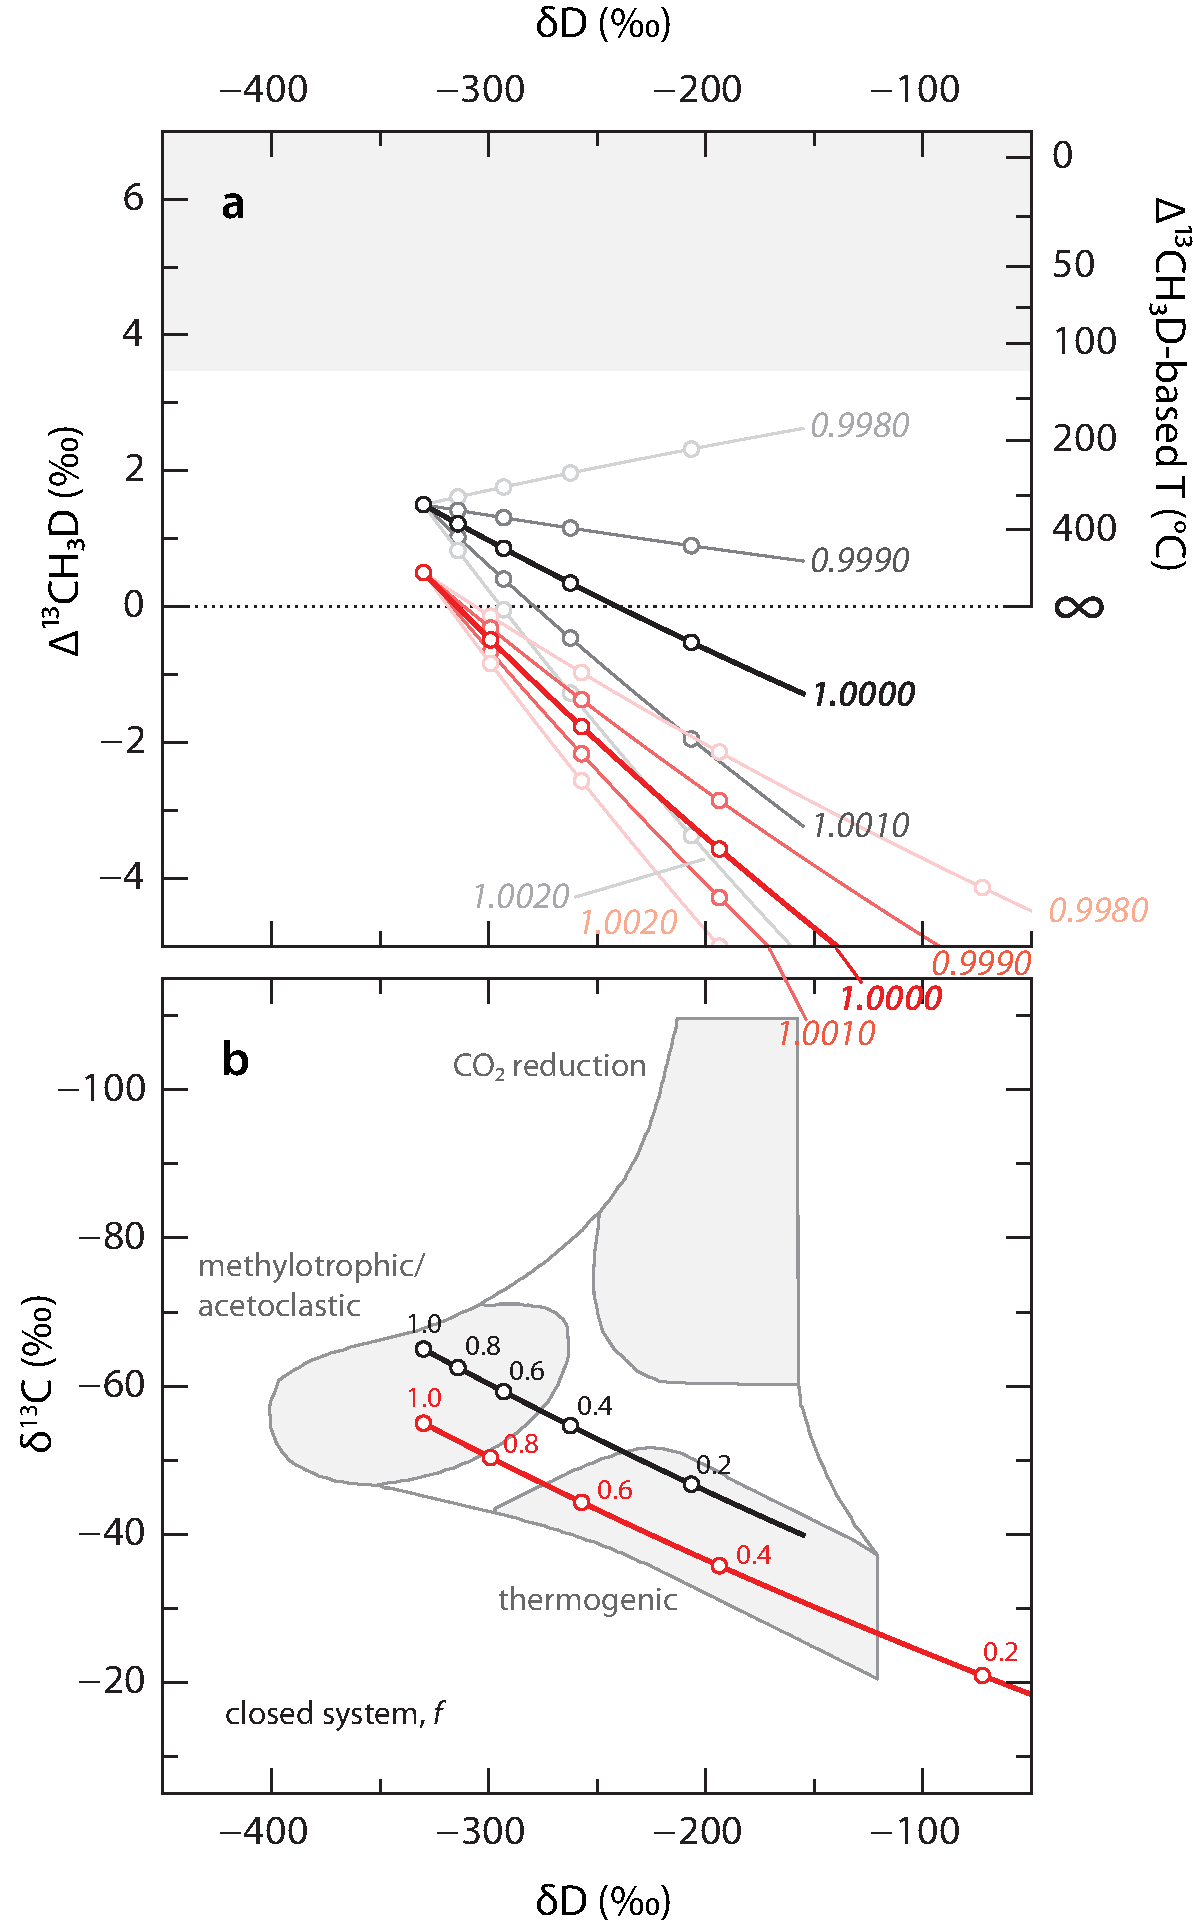
\includegraphics[width=0.5\textwidth]{figures/Fig4.3}
	\caption[Trajectories for isotope/isotopologue ratios of methane oxidized in a closed system]{Modeled changes in \textbf{(a)}
		Δ\textsuperscript{13}CH\textsubscript{3}D vs.\ δD and \textbf{(b)}
		δ\textsuperscript{13}C vs.\ δD of residual methane during aerobic methane
		oxidation under closed system conditions. Solid lines represent model
		predictions (from \mrefs[]{Eqns.}{eqn:4:13}, \ref{eqn:4:16}, and~\ref{eqn:4:20}) based on the calculated
		weighted-average carbon- and hydrogen-isotope fractionation factors for
		each set of experiments (black, 30~°C; red, 37~°C) as listed in \autoref{tab:4:1}
		and shown in \autoref{fig:4:1}. Labels in \emph{italics} in panel (a) represent $\gamma$
		values. Circles are marked at intervals of 0.2 in \emph{f}, the fraction
		of initial methane remaining, and labeled in panel (b). For visual
		clarity, the models were initialized at slightly different
		δ\textsuperscript{13}C and Δ\textsuperscript{13}CH\textsubscript{3}D
		values. The initial isotope values were chosen for illustrative purposes
		only and do not represent any particular natural sample; however, the
		chosen values are typical of modern microbial methane generated in
		wetland and lake sediments. Following \textcite{Wang++_2015_S}, the gray field
		in panel (a) represents the temperature range within which microbial
		life has been shown to occur \parencite{Takai++_2008_PNAS}, and the gray fields
		in panel (b) represent empirical methane source fields suggested by
		\textcite{Whiticar_1999_CG}.}
	\label{fig:4:3}
\end{SCfigure*}


In our batch culture experiments, the
Δ\textsuperscript{13}CH\textsubscript{3}D value of residual methane
decreased with progressive oxidation (\autoref{tab:4:1}). The weighted average $\gamma$
values determined for the both the 30~°C experiment (1.0005 ± 0.0006,
2$\sigma$) and the 37~°C experiment (1.0000 ± 0.0014) are indistinguishable
from unity. Thus, the results of this study indicate that the overall
kinetic fractionation factor for
\textsuperscript{13}CH\textsubscript{3}D/\textsuperscript{12}CH\textsubscript{4}
can be closely approximated as the product of the carbon and hydrogen
isotopic fractionation factors (i.e., \textsuperscript{13--D}$\alpha$ $\approx$
\textsuperscript{13}$\alpha$ $\cdot$ \textsuperscript{D}$\alpha$). This product rule can be
used to model the Δ\textsuperscript{13}CH\textsubscript{3}D value
resulting from aerobic methane oxidation. If a higher level of
prediction is necessary, precise constraints on primary and secondary $\alpha$
and $\gamma$ values are required (see \autoref{sec:4:13ch3d-fractionation} and discussion below).

Given low enough $\gamma$ values (depending on \textsuperscript{13}$\alpha$ and
\textsuperscript{D}$\alpha$), the Δ\textsuperscript{13}CH\textsubscript{3}D
value may actually \emph{increase} over the course of the reaction in a
closed system such as a batch culture. The break-even condition, under
which Δ\textsuperscript{13}CH\textsubscript{3}D does not change during a closed system process, occurs when
\(\gamma = \left.{\left({}_{}^{13}\alpha +{}_{}^{\mathrm{D}}\alpha - 1 \right)}\middle/{\left({}_{}^{13}\alpha \cdot{}_{}^{\mathrm{D}}\alpha \right)}\right.\).
For the 30 and 37~°C experiments, the break-even $\gamma$ values are 0.9986 and
0.9943, respectively. These values are substantially less than those
determined experimentally above (the latter by a considerable $-$0.0057 or
$-$5.7‰). Therefore, it should not be assumed that
Δ\textsuperscript{13}CH\textsubscript{3}D values are unaffected by
closed system methane oxidation. Otherwise, the apparent
Δ\textsuperscript{13}CH\textsubscript{3}D temperature may be
substantially overestimated or become imaginary, as shown in \mrefs[a]{Fig.}{fig:4:3}.

There is no \emph{a priori} reason that $\gamma$ must be close to
unity.\footnote{For example, when methane effuses through a small
	orifice, $\gamma$ (when defined as the ratio of the isotopologue
	fractionation factor for
	\textsuperscript{13}CH\textsubscript{3}D/\textsuperscript{12}CH\textsubscript{4}
	to the product of those for
	\textsuperscript{13}CH\textsubscript{4}/\textsuperscript{12}CH\textsubscript{4}
	and
	\textsuperscript{12}CH\textsubscript{3}D/\textsuperscript{12}CH\textsubscript{4})
	will not be unity. From the kinetic theory of gases, the rate of
	effusion of an isotopologue is proportional to
	(mass)\textsuperscript{$-$1/2}, such that $\gamma$ = 1.00174. Escaping methane
	will have lower (lighter) δ\textsuperscript{13}C and δD, but
	\emph{higher} Δ\textsuperscript{13}CH\textsubscript{3}D, than the
	residual methane. For a more thorough discussion, readers are referred
	to \textcite{Eiler+Schauble_2004_GCA}.} The $\gamma$ factor as defined in \autoref{sec:4:13ch3d-fractionation}
is empirically useful in that it is a single number that expresses the
reactivity of \textsuperscript{13}CH\textsubscript{3}D relative to the
other isotopologues. Because \textsuperscript{13}CH\textsubscript{3}D
can react by two nonidentical hydrogen-abstraction reactions (\mrefs[]{Reactions}{eqn:4:8} and \ref{eqn:4:9}), the $\gamma$ value expresses the summation of the products of the
hydrogen-isotope effects (\textsuperscript{D}$\alpha$\textsubscript{p} and
\textsuperscript{D}$\alpha$\textsubscript{s}) and the ``clumped isotopologue
effects'' ($\gamma$\textsubscript{p} and $\gamma$\textsubscript{s}) for D in both
primary and secondary sites:
\(\gamma \cdot{}_{}^{\mathrm{D}}\alpha = \frac{1}{4} \cdot \gamma_{\mathrm{p}} \cdot{}_{}^{\mathrm{D}}\alpha_{\mathrm{p}} + \frac{3}{4} \cdot \gamma_{\mathrm{s}} \cdot{}_{}^{\mathrm{D}}\alpha_{\mathrm{s}}\).
A conceptual exercise helpfully illustrates the relative weighting of D-
vs.\ H-abstraction reactions expressed in the $\gamma$ factor. Assuming
\textsuperscript{D}$\alpha$\textsubscript{p} = 0.02 and
\textsuperscript{D}$\alpha$\textsubscript{s} = 0.9 (from \autoref{sec:4:fractionation-of-methane-13c12c-and-dh-ratios}), and $\gamma$ =
0.9990 (i.e., $-$1‰ from unity, which is at the lower edge of 2$\sigma$
uncertainty on the weighted average $\gamma$ values for the experiments shown
in \autoref{tab:4:1}), then \textsuperscript{D}$\alpha$ = 0.68 and
\(0.6786 = 0.0050 \cdot \gamma_{\mathrm{p}} + 0.6750 \cdot \gamma_{\mathrm{s}}\).
Assigning a value to either $\gamma$\textsubscript{p} or $\gamma$\textsubscript{s}
would constrain the other; hence, two extreme cases can be considered:
(\emph{i}) if $\gamma$\textsubscript{s} = 1, then $\gamma$\textsubscript{p} = 0.86; or
alternatively (\emph{ii}) if $\gamma$\textsubscript{p} = 1, then
$\gamma$\textsubscript{s} = 0.9990. The former case requires a large primary
clumped isotopologue effect because proportionally very few
\textsuperscript{13}CH\textsubscript{3}D (and
\textsuperscript{12}CH\textsubscript{3}D) molecules react through direct
D-abstraction rather than H-abstraction (see \autoref{sec:4:fractionation-of-methane-13c12c-and-dh-ratios}), whereas the
latter requires only a much smaller secondary clumped isotopologue
effect on H-abstraction from \textsuperscript{13}CH\textsubscript{3}D to
explain a $\gamma$ value that deviates slightly from unity. Although
insufficient constraints on either $\gamma$\textsubscript{p} or
$\gamma$\textsubscript{s} are currently available, this exercise indicates that
a small secondary clumped isotopologue effect (i.e., $\gamma$\textsubscript{s}
$\neq$ 1 but is very close) could exist, but may be hardly detectable. Given
the uncertainties surrounding experimental determinations of
\textsuperscript{D}$\alpha$\textsubscript{p} and
\textsuperscript{D}$\alpha$\textsubscript{s} (discussed in \autoref{sec:4:fractionation-of-methane-13c12c-and-dh-ratios}),
accurate values of $\gamma$\textsubscript{p} and $\gamma$\textsubscript{s} cannot yet
be assigned. For geochemical applications, the $\gamma$ factor is at present
best used as an empirically-fitted parameter, similar to the manner in
which the overall D/H fractionation factor \textsuperscript{D}$\alpha$ is
typically treated.

Irrespective of the exact magnitude of the $\gamma$ factor, it is clear that
Δ\textsuperscript{13}CH\textsubscript{3}D becomes less clumped with
progressive oxidation in a closed system under the growth conditions
tested in this study. Because of the consistency of our
\textsuperscript{D}$\varepsilon$/\textsuperscript{13}$\varepsilon$ results with previous
experiments with organisms also using pMMO and/or sMMO (\mrefs[a]{Fig.}{fig:4:2}), it is
not unreasonable to expect similar results on
Δ\textsuperscript{13}CH\textsubscript{3}D values for methane oxidation
by other strains of aerobic methanotrophic bacteria.

As mentioned above (\autoref{sec:4:fractionation-of-methane-13c12c-and-dh-ratios}), a possible explanation for the
differences in the hydrogen isotopic fractionation factor for the
experiments at the two temperatures relates to partial expression of
equilibrium isotope effects in one or both experiments. Evidence against
this explanation derives from the observation that
Δ\textsuperscript{13}CH\textsubscript{3}D values of residual methane in
both experiments follow the predictions of the product rule (i.e., $\gamma$
values are \textasciitilde{}1); therefore it is unlikely that there is a
greater degree of C--H bond re-equilibration during the course of
reaction in one experiment over another. Thus, clumped isotopologue data
also assist in diagnosing presence or absence of isotope exchange during
enzymatic abstraction of H from methane by MMO, and are consistent with
a minor (not detectable) degree of reversibility for this process. The
minor degree of reversibility indicated by the data for aerobic methane
oxidation here contrasts sharply with the anaerobic oxidation of methane
(AOM), an oxidation process in which much greater degrees of
reversibility have been demonstrated using carbon and hydrogen isotopes
\parencite{Holler++_2011_PNAS,Yoshinaga++_2014_NG}. The environmental
implications are discussed in \autoref{sec:4:13ch3d-as-an-environmental-tracer-of-methane-sink-processes}.

\subsection{Implications for biogeochemical systems
}\label{sec:4:implications-for-biogeochemical-systems}

\subsubsection{Methane isotope and isotopologue fractionation in open
	systems}\label{sec:4:methane-isotope-and-isotopologue-fractionation-in-open-systems}


\begin{SCfigure*}
	\centering
	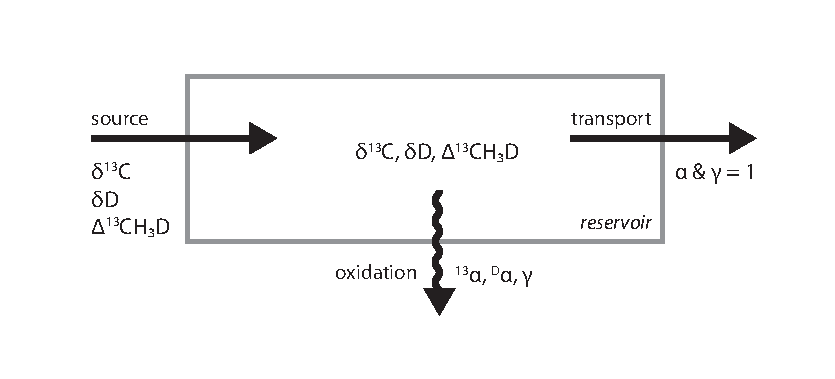
\includegraphics[width=0.7\textwidth]{figures/Fig4.4}
	\caption[Box model for a methane reservoir with transport and oxidation]{Representation of a model open system in which methane
		is transported in and out via advection, and in which aerobic methane
		oxidation is also occurring. The fractional contribution of oxidation to
		the total sinks is $\varphi$\textsubscript{ox}. See \autoref{fig:4:5} and discussion in
		\autoref{sec:4:methane-isotope-and-isotopologue-fractionation-in-open-systems}.}
	\label{fig:4:4}
\end{SCfigure*}


In closed systems, e.g., batch cultures, no steady state is obtained
because of the lack of mass transfer to replenish the methane consumed
by methane oxidation. However, in natural systems operating close to
steady state, there is replenishment of methane from lateral transport
or diffusion, as well as methanogenesis, and there may be multiple
sinks, including methane oxidation and mass transport (\autoref{fig:4:4}).

Experimental alternatives to batch cultures, namely flow-through
bioreactors (chemostats), have been used to more directly approach the
calibration of isotopic fractionation factors due to microbial
metabolism in natural settings. For example, \textcite{Templeton++_2006_GCA}
grew pure and mixed cultures of aerobic methanotrophs in chemostats to
determine the carbon isotope fractionation between methane and product
methanol as a function of environmental and physiological conditions. In
such an open system, there is a constant influx of reactant methane,
which at steady state is balanced by the sum of methane oxidation and
methane carried in the effluent out of the bioreactor (i.e., dilution).


\begin{SCfigure*}
	\centering
	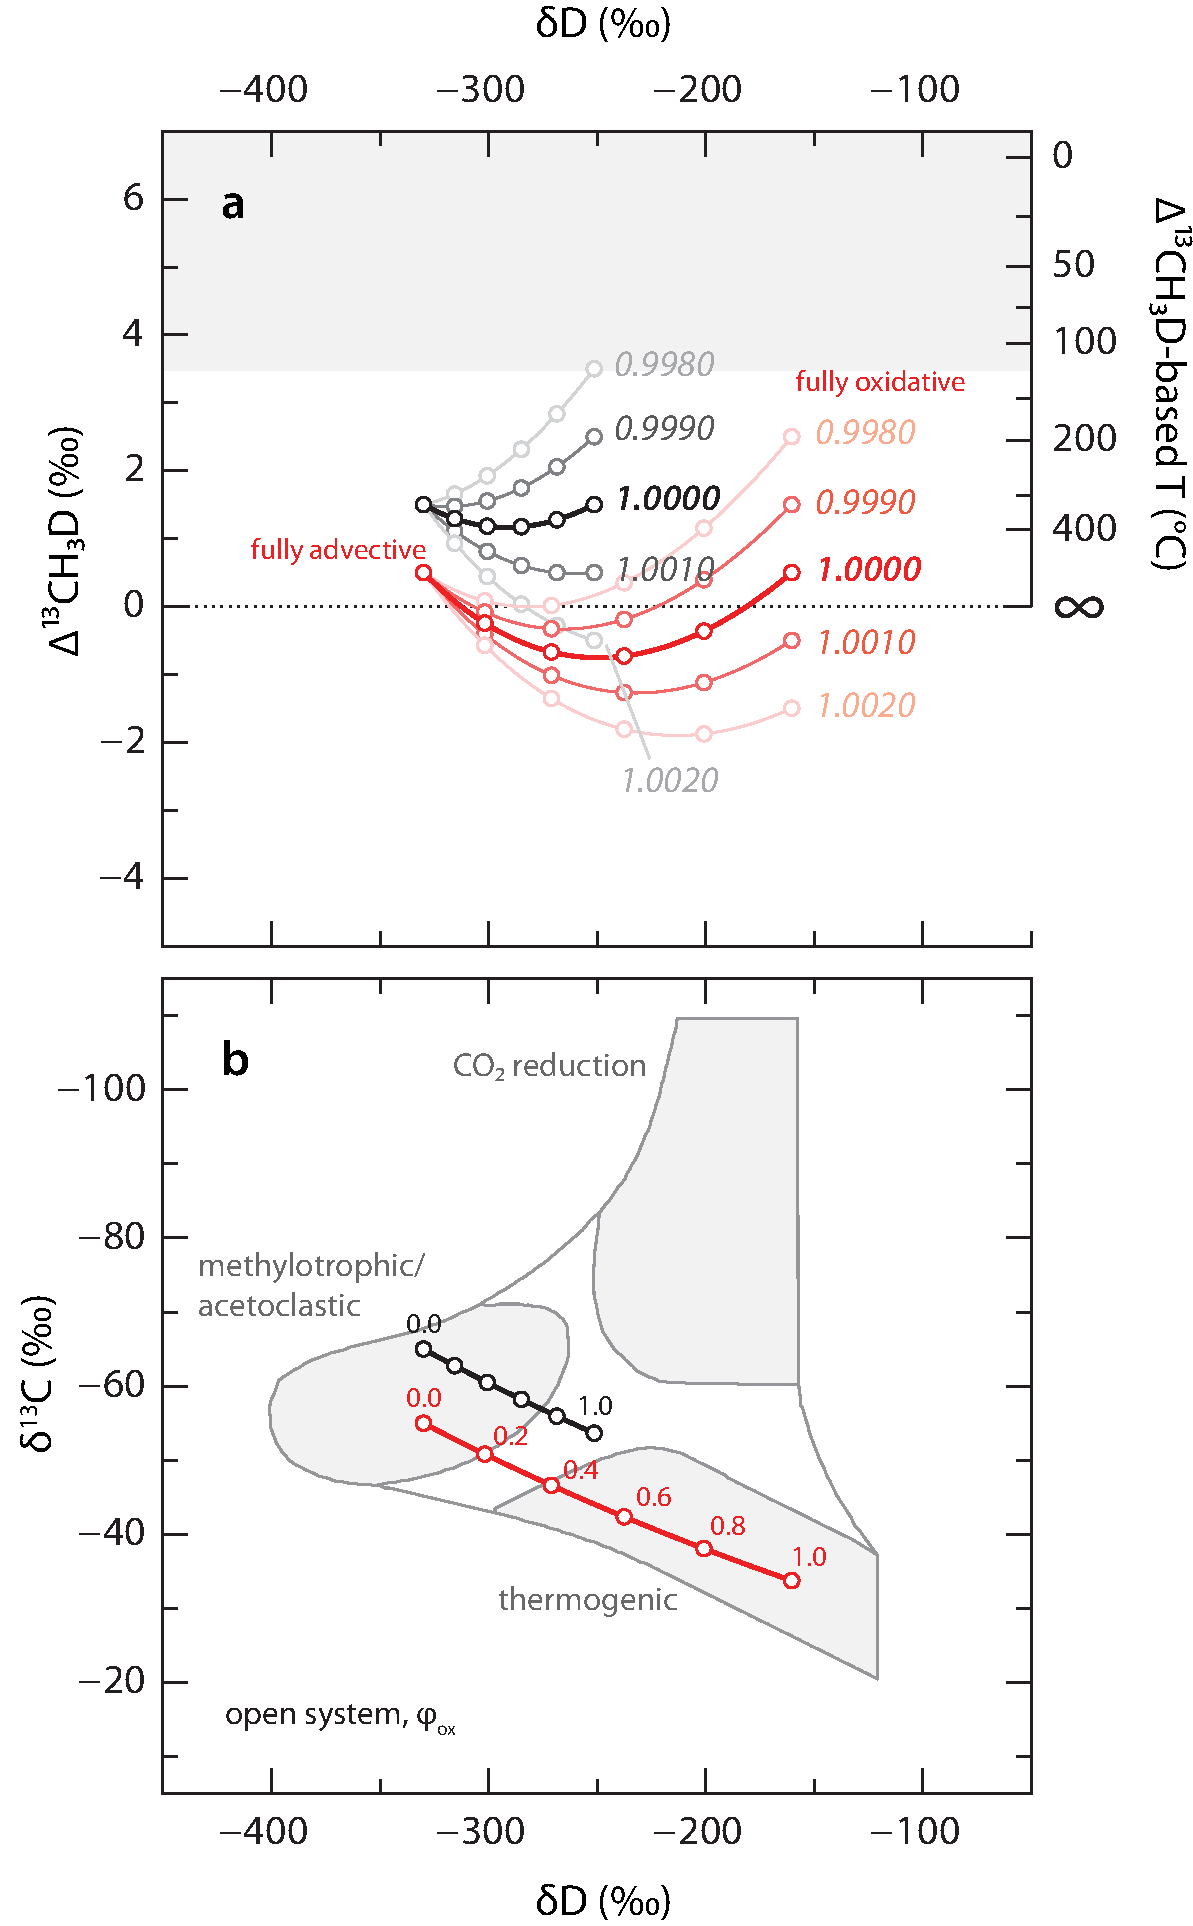
\includegraphics[width=0.5\textwidth]{figures/Fig4.5}
	\caption[Trajectories for isotope/isotopologue ratios of methane oxidized in an open system]{Modeled steady-state values of \textbf{(a)}
		Δ\textsuperscript{13}CH\textsubscript{3}D vs.\ δD and \textbf{(b)}
		δ\textsuperscript{13}C vs.\ δD of methane in an open system (\autoref{fig:4:4})
		consisting of a single source and two sinks (aerobic methane oxidation
		and advection). Advection is assumed to be non-fractionating. Lines were
		modeled using \mrefs[]{Eqns.}{eqn:4:22} and \ref{eqn:4:23}, and the same fractionation factors for
		aerobic methane oxidation as for those shown with the same line style in
		\autoref{fig:4:2}. Labels in \emph{italics} in panel (a) represent $\gamma$ values
		associated with aerobic methane oxidation. Circles are marked at
		intervals of 0.2 in $\varphi$\textsubscript{ox}, the fraction of methane removed
		via oxidation, ranging from fully advective ($\varphi$\textsubscript{ox} = 0) to
		fully oxidative ($\varphi$\textsubscript{ox} = 1), and labeled in panel (b).
		When $\varphi$\textsubscript{ox} = 0, the isotopic composition of methane in the
		reservoir is identical to that of the source. For visual clarity, the
		calculations were performed for slightly different
		δ\textsuperscript{13}C and Δ\textsuperscript{13}CH\textsubscript{3}D
		values of input methane. For description of shaded fields, see the
		caption for \autoref{fig:4:3}.}
	\label{fig:4:5}
\end{SCfigure*}

In the simple limiting case where the fraction of methane removed by
oxidation approaches 100\% (i.e., no methane escapes the system intact),
there is effectively one sink of methane, with fractionation factors
\textsuperscript{13}$\alpha$, \textsuperscript{D}$\alpha$, and $\gamma$ accompanying the
removal process. At steady state, the isotopic values of methane in the
bioreactor would be δ\textsuperscript{13}C =
(δ\textsuperscript{13}C\textsubscript{in} + 1) \big/ \textsuperscript{13}$\alpha$ $-$
1 and δD = (δD\textsubscript{in} + 1) \big/ \textsuperscript{D}$\alpha$ $-$ 1, where
δ\textsubscript{in} represents the isotopic composition of the influent
methane. For \textsuperscript{13}CH\textsubscript{3}D, it can be shown
that
\begin{equation}\label{eqn:4:21}
\Delta_{}^{\mathrm{13}}{\mathrm{C}\mathrm{H}_{\mathrm{3}}\mathrm{D}} = {\Delta_{}^{\mathrm{13}}{\mathrm{C}\mathrm{H}_{\mathrm{3}}\mathrm{D}}}_{\mathrm{\text{in}}} - \ln\gamma\
\end{equation}
as presented in \textcite{Joelsson++_2015_ACPD}. Since $\gamma$ $\approx$ 1, this expression can
be approximated by Δ\textsuperscript{13}CH\textsubscript{3}D~= Δ\textsuperscript{13}CH\textsubscript{3}D\textsubscript{in}~$- (\gamma - 1$).
In our batch culture experiments at 30 and 37~°C, respectively,
weighted-average values for ($\gamma - 1$) of +0.5 ± 0.3‰ and 0.0 ± 0.7‰ (1$\sigma$)
were obtained (\autoref{tab:4:1}). Although steady-state experiments were not
conducted in the current study, if it is assumed that these values are
also characteristic of true open-system isotopologue fractionation
factors, then the above expression can be used to place bounds on the
isotopologue composition of methane in the limiting case outlined above.
Examples of the calculated methane isotopic/isotopologue compositions
are shown for model scenarios in \mrefs[a]{Fig.}{fig:4:5} (corresponding to the endmember
labeled ``fully oxidative'' on each curve).

\mrefs[]{Equation}{eqn:4:21} also shows that in a system at steady state where methane is
solely removed by one process (here, oxidation), the
Δ\textsuperscript{13}CH\textsubscript{3}D value is determined solely by
the Δ\textsuperscript{13}CH\textsubscript{3}D value of the methane
source and the $\gamma$ factor, in contrast to closed systems where
Δ\textsuperscript{13}CH\textsubscript{3}D of residual methane is
influenced also by the isotopic fractionations for bulk
\textsuperscript{13}C/\textsuperscript{12}C and D/H. However, in more
complex systems with multiple removal processes and associated
fractionation factors, the partitioning of flows among the removal
processes must be considered \parencite{Hayes_2001_RiMG}.

One example of such an open system is shown in \autoref{fig:4:4}. Here, methane is
carried into the system via advection, and removed by both advection and
oxidation. Oxidation of methane has associated fractionation factors
\textsuperscript{13}$\alpha$, \textsuperscript{D}$\alpha$, and $\gamma$, whereas transport
processes are assumed to cause no fractionation \parencite{Alperin++_1988_GBC},
i.e., values of $\alpha$ and $\gamma$ are unity. The fraction of methane removed via
oxidation, $\varphi$\textsubscript{ox}, describes the partitioning of flows
among the two methane sinks. It can be shown that at steady state, the
hydrogen isotopic composition of the methane in the reservoir is \parencite{Hayes_2001_RiMG}:
\begin{equation}\label{eqn:4:22}
\mathrm{\text{δD}} = \ \frac{\mathrm{\text{δD}}_{\mathrm{\text{in}}} + 1}{1 + \varphi_{\mathrm{\text{ox}}}\left({}_{}^{\mathrm{D}}\alpha - 1 \right)} - 1
\end{equation}

An analogous equation (not shown) describes the carbon isotopic
composition of methane in this system at steady state. When the
δ\textsuperscript{13}C and δD values are plotted against each other, it
can be seen that the trajectory describing the continuum between the
fully-advective ($\varphi$\textsubscript{ox} = 0) and fully-oxidative
($\varphi$\textsubscript{ox} = 1) endmembers is slightly curved (though
approximately linear at most scales of interest, \mrefs[b]{Fig.}{fig:4:5}).

For this system, unlike in the simple fully-oxidative case described by \autoref{eqn:4:21}, the abundance of \textsuperscript{13}CH\textsubscript{3}D is affected not only by the $\gamma$ value, but also by
the \textsuperscript{13}$\alpha$ and \textsuperscript{D}$\alpha$ values:
\begin{equation}\label{eqn:4:23}
\Delta_{}^{\mathrm{13}}{\mathrm{C}\mathrm{H}_{\mathrm{3}}\mathrm{D}} = {\Delta_{}^{\mathrm{13}}{\mathrm{C}\mathrm{H}_{\mathrm{3}}\mathrm{D}}}_{\mathrm{\text{in}}} - \ln\frac{1 + \varphi_{\mathrm{\text{ox}}}\left( \gamma \cdot{}_{}^{13}\alpha \cdot{}_{}^{\mathrm{D}}\alpha - 1 \right)}{\left( 1 + \varphi_{\mathrm{\text{ox}}}\left({}_{}^{13}\alpha - 1 \right) \right)\left( 1 + \varphi_{\mathrm{\text{ox}}}\left({}_{}^{\mathrm{D}}\alpha - 1 \right) \right)}\ 
\end{equation}

This results in a parabolic curve connecting the fully-advective and
fully-oxidative endmembers (\mrefs[a]{Fig.}{fig:4:5}). For aerobic methane oxidation, the
curvature on \mrefs[a]{Fig.}{fig:4:5} is always expected to be concave up, because both
the \textsuperscript{13}$\alpha$ and \textsuperscript{D}$\alpha$ values are less than
unity. The relative position of the endmembers in
Δ\textsuperscript{13}CH\textsubscript{3}D space is determined by the $\gamma$
value. When $\varphi$\textsubscript{ox} = 1, \autoref{eqn:4:23} reduces to \autoref{eqn:4:21}.

\subsubsection{\texorpdfstring{Δ\textsuperscript{13}CH\textsubscript{3}D as
		an environmental tracer of methane sink
		processes}{Δ13CH3D as an environmental tracer of methane sink processes}}\label{sec:4:13ch3d-as-an-environmental-tracer-of-methane-sink-processes}

Both biological and chemical processes are important sinks in the
methane budget. In terrestrial ecosystems and oxygenated marine water
columns, aerobic methanotrophy dominates, whereas in sulfate-rich marine
sediments and gas seeps, anaerobic consumption of methane becomes
important \parencite{Cicerone+Oremland_1988_GBC,Reeburgh_2007_CR,Valentine_2011_ARMar,Boetius+Wenzhoefer_2013_NG}. In the atmosphere, the primary sink
(\textasciitilde{}90\%) is the reaction with tropospheric OH, with small
contributions from microbial oxidation in soils, loss to stratosphere,
and reaction with tropospheric Cl \parencite{Kirschke++_2013_NG}.

These methane-consuming processes impart distinct carbon- and
hydrogen-isotopic fractionations. In general, biological processes
(including aerobic methane oxidation, anaerobic oxidation of methane,
and nitrite-dependent anaerobic methane oxidation) have
\textsuperscript{D}$\varepsilon$/\textsuperscript{13}$\varepsilon$ ratios between 6 and 15,
whereas the atmospheric sinks, CH\textsubscript{4} + OH and
CH\textsubscript{4} + Cl, have
\textsuperscript{D}$\varepsilon$/\textsuperscript{13}$\varepsilon$ ratios \textasciitilde{}58
and \textasciitilde{}5.5, respectively (\autoref{tab:4:2}). The consistent and
sizable differences in isotopic behavior among the two atmospheric
processes vs.\ biological processes is useful for constraining the
balance of different sources and sinks of methane \parencite[e.g.,][]{Kai++_2011_N,Rigby++_2012_JGR,Whiticar+Schaefer_2007_PTRSA}.

The behavior of methane clumped isotopologues in atmospheric reactions
has also been studied. Recently, \textcite{Joelsson++_2014_CPL} and \textcite{Joelsson++_2016_ACP} reported the fractionation factor for
\textsuperscript{13}CH\textsubscript{3}D in relative-rate experiments on
the reactions of Cl and OH, respectively. Their experiments were
conducted with mixtures of \textsuperscript{12}CH\textsubscript{4} and
\textsuperscript{13}CH\textsubscript{3}D (and also
\textsuperscript{12}CH\textsubscript{3}D in the OH study). Based on
their measurements, the $\gamma$ value associated with methane oxidation by Cl
was 0.980 ± 0.019, and by OH was 0.978 ± 0.028 (2$\sigma$, \autoref{tab:4:2}). The $\gamma$
value for Cl oxidation is slightly less than unity, implying that less
of the \textsuperscript{13}CH\textsubscript{3}D is oxidized than would
be predicted by the product rule, whereas the $\gamma$ value for OH oxidation
is within error of unity. However, the uncertainty on calculated $\gamma$
values is large (ca.\ 20 to 30‰) due to limitations associated with the
experimental setup and detection technique. Because
Δ\textsuperscript{13}CH\textsubscript{3}D in the environment has a ca.
10‰ range \parencite{Wang++_2015_S}, more precise isotopologue-specific
measurements of methane in experiments conducted at natural abundance
will be necessary in order to constrain clumped isotopologue
fractionations in atmospheric contexts. These experiments have been
conducted, and the results are reported in a companion article
\parencite{Whitehill++_2017_GCA}; a summary of their results are shown in \autoref{tab:4:1}.%\hyperref[tab:4:1]{Tables \ref*{tab:4:1}} and \ref{tab:4:2}.

\begin{table}[t]
		\caption[Comparison of \textsuperscript{D}$\varepsilon$/\textsuperscript{13}$\varepsilon$ and $\gamma$ values for various methane sinks]{Comparison of experimentally-determined ratios of carbon- and
			hydrogen-isotope fractionation factors
			(\textsuperscript{D}$\varepsilon$/\textsuperscript{13}$\varepsilon$) and
			\textsuperscript{13}CH\textsubscript{3}D fractionation factors ($\gamma$) for
			different methane sink processes. Uncertainties quoted are ±2$\sigma$ or 95\%
			confidence interval.}
		\label{tab:4:2}
	\centering
	\begin{threeparttable}
		\begin{tabular}{lll}
			\toprule
			& \textsuperscript{D}$\varepsilon$/\textsuperscript{13}$\varepsilon$ & $\gamma$\tabularnewline
			\midrule
			& &\tabularnewline
			\multicolumn{3}{l}{\emph{Aerobic methane oxidation}}\tabularnewline
			Previous work\tnote{a} & 5.9 to 14.9 &\tabularnewline
			This study\tnote{b} & 9.14 ± 0.14 & 1.0004 ±
			0.0006\tabularnewline
			& &\tabularnewline
			\multicolumn{3}{l}{\emph{Anaerobic oxidation of methane (AOM)}}\tabularnewline
			\textcite{Holler++_2009_EMR} & 6.4 to 8.5 &\tabularnewline
			& &\tabularnewline
			\multicolumn{3}{l}{\emph{Nitrite-dependent anaerobic methane oxidation}}\tabularnewline
			\textcite{Rasigraf++_2012_GCA} & 7.8 ± 0.8 &\tabularnewline
			& &\tabularnewline
			\multicolumn{3}{l}{\emph{CH\textsubscript{4} + OH}} \tabularnewline
			\textcite{Saueressig++_2001_JGR} & 58.5 ± 6.6 &\tabularnewline
			\citeauthor{Joelsson++_2016_ACP} (\cite*{Joelsson++_2015_ACPD,Joelsson++_2016_ACP}) & & 0.980 ± 0.038\tabularnewline
			\textcite{Whitehill++_2017_GCA} & 41.3 ± 8.3 & 0.9997 ± 0.0012\tabularnewline
			& &\tabularnewline
			\multicolumn{3}{l}{\emph{CH\textsubscript{4} + Cl}}\tabularnewline
			\textcite{Tyler++_2000_GRL} & 5.51 &\tabularnewline
			\citeauthor{Saueressig++_1995_GRL} (\cite*{Saueressig++_1995_GRL,Saueressig++_1996_GRL}) & 5.50 &\tabularnewline
			\textcite{Feilberg++_2005_IJChemKin} & 5.65 &\tabularnewline
			\textcite{Joelsson++_2014_CPL} & & 0.978 ± 0.051\tabularnewline
			\textcite{Whitehill++_2017_GCA} & 5.56 & 0.9965 ± 0.0007\tabularnewline
			& &\tabularnewline
			\bottomrule
		\end{tabular}
		\begin{tablenotes}
			\item[a] See caption of \mrefs[a]{Fig.}{fig:4:2} for references. Also see
			\textcite{Rasigraf++_2012_GCA} for a compilation of \textsuperscript{13}$\varepsilon$ and
			\textsuperscript{D}$\varepsilon$ values determined for biological methane oxidation
			in cultures and in the environment.
			\item[b] Derived from linear regression
			(\textsuperscript{D}$\varepsilon$/\textsuperscript{13}$\varepsilon$, \mrefs[a]{Fig.}{fig:4:2}) or weighted
			average ($\gamma$) of all timepoints in both experiments in \autoref{tab:4:1}.
		\end{tablenotes}
	\end{threeparttable}

\end{table}


In the present study, $\gamma$ values for aerobic methane oxidation were
determined (1.0004 ± 0.0006, 2$\sigma$, \autoref{tab:4:2}). These values indicate that
the abstraction of H from methane by methane monooxygenase is associated
with little to no reversibility (see discussion in \autoref{sec:4:fractionation-of-13ch3d}). This
interpretation is consistent with the strong energetic favorability of
methane oxidation to methanol and downstream products in the presence of
abundant O\textsubscript{2}, a strong electron acceptor \parencite{Cicerone+Oremland_1988_GBC,Hanson+Hanson_1996_MMBR}.

The new experimental constraints on clumped isotopologue fractionation
during aerobic methane oxidation also afford an opportunity to briefly
evaluate whether aerobic methane oxidation has influenced methane
clumped isotopologue data available in the literature from various
environments. In particular, because methane oxidation demonstrably
produces nonequilibrium clumped isotopologue signatures in both closed
and open systems considered in this study (\mrefs{Figs.}{fig:4:3} and \ref{fig:4:5}, respectively),
the out-of-equilibrium clumped isotopologue signatures in samples from
Upper and Lower Mystic Lakes (Massachusetts, USA), Swamp Y
(Massachusetts, USA), and The Cedars (California, USA) are considered
again here \parencite{Wang++_2015_S}, as well as a sample from a pond at
Caltech for which a related parameter, the Δ\textsubscript{18} value,
was found to be in disequilibrium \parencite{Stolper++_2015_GCA}. At Upper
Mystic Lake (a 20-m deep seasonally-stratified freshwater lake), bubble
traps were deployed \textasciitilde{}2 m above the lake floor; the
deployment of traps at such deep depths, into the oxygen-depleted
hypolimnion \parencite{Peterson_2005_thesis}, was designed to minimize the possibility
of aerobic methane oxidation \parencite{Wang++_2015_S}. At Lower Mystic Lake
(a 24-m deep meromictic density-stratified lake), the monimolimnion
(from which the reported sample was taken) is anoxic \parencite{Wang++_2015_S}, rendering aerobic methane oxidation unlikely. For Swamp Y and the
Caltech pond, the redox state of the sediments from which the methane
bubbles were stirred and extracted is unknown. At The Cedars, the
extremely high levels of H\textsubscript{2} in gases exsolving from the
springs maintains O\textsubscript{2} at vanishingly low levels \parencite[near the
lower bound of H\textsubscript{2}O stability;][]{Morrill++_2013_GCA}.
Taken together, all methane samples from these four sites exhibit narrow
ranges of δ\textsuperscript{13}C values between $-$59‰ and $-$71‰ and δD
values between $-$265‰ and $-$342‰, but carry a wide range of nonequilibrium
Δ\textsuperscript{13}CH\textsubscript{3}D values (from $-$3.4‰ to +3.2‰)
that are consistent within sites but significantly different between
sites \parencite{Wang++_2015_S}, and exhibit isotopologue patterns that do not
discernably resemble those depicted in \mrefs[]{Figs.}{fig:4:3} and \ref{fig:4:5}. Thus, although
aerobic methane oxidation cannot be fully discounted at these four
sites, the experimental constraints provided in the current study do not
contraindicate the assumptions made by \textcite{Wang++_2015_S} and are
consistent with the hypothesis that nonequilibrium
Δ\textsuperscript{13}CH\textsubscript{3}D values in microbial methane in
the environment and in methanogenic cultures studied to date originate
primarily from intrinsic isotopologue effects during the assembly of
C--H bonds during methanogenesis \parencite{Stolper++_2015_GCA,Wang++_2015_S}.

Alternative biological mechanisms for methane oxidation are also
important in the environment. Of particular interest is the
sulfate-dependent anaerobic oxidation of methane (AOM), which is a major
sink of methane in anoxic marine sediments \parencite{Reeburgh_1976_EPSL}. This
process operates via a very different biochemical pathway from that used
by aerobic methanotrophs. While the biochemistry of AOM has not been
fully characterized, it is likely that the enzymatic pathway of AOM is
the reverse of methanogenesis, and involves the same or similar key
enzymes (e.g., methyl-coenzyme M reductase) for addition or removal of H
from single-carbon compounds \parencite{Scheller++_2010_N}. Previously, it was
found that as the reversibility of methanogenesis decreased (controlled
in part by levels of bioavailable H\textsubscript{2}), both the δD and
Δ\textsuperscript{13}CH\textsubscript{3}D values of the generated
methane became lower or more negative \parencite{Wang++_2015_S}; similar
behavior was found in Δ\textsubscript{18} \parencite{Stolper++_2014_S,Stolper++_2015_GCA}. From incubations of enrichment cultures of
microbial consortia performing AOM, \textcite{Holler++_2009_EMR} determined
substantial kinetic isotope fractionations associated with this process
(\textsuperscript{13}$\varepsilon$ = $-$12‰ to $-$36‰ and \textsuperscript{D}$\varepsilon$ = $-$100‰
to $-$230‰). The negative D/H fractionation factor results in the residual
methane becoming enriched in D. Because of the demonstrated high levels
of reversibility of AOM \parencite{Holler++_2011_PNAS} and the re-equilibration
of \textsuperscript{13}C/\textsuperscript{12}C ratios between methane
and inorganic carbon at the sulfate-methane transition zone \parencite{Yoshinaga++_2014_NG}, it seems reasonable to speculate that AOM may produce
clumped isotope signatures distinct from those of methanogenesis
\parencite{Stolper++_2015_GCA}. In particular, the expression of a combination
of kinetic and equilibrium isotope effects may be observed, such that
the observed Δ\textsuperscript{13}CH\textsubscript{3}D value may lie
between that predicted by the product rule and that predicted for
thermodynamic equilibrium. If so, then measurement of
Δ\textsuperscript{13}CH\textsubscript{3}D may provide a way to
differentiate between AOM and aerobic methanotrophy. Alternatively, if
AOM also generates Δ\textsuperscript{13}CH\textsubscript{3}D
approximating the product rule, then the agreement of
\textsuperscript{D}$\varepsilon$/\textsuperscript{13}$\varepsilon$ between AOM \parencite{Holler++_2009_EMR} and aerobic methanotrophs (\autoref{tab:4:2}) suggests that potentially,
microbially-mediated oxidation of methane produces only a small and
predictable range of clumped isotopologue fractionations.

Another process, the recently-identified nitrite-dependent anaerobic
methane oxidation \parencite{Ettwig++_2010_N}, may also be
environmentally-relevant, though its global prevalence has yet to be
established. The bacterium Candidatus \emph{Methylomirabilis oxyfera}
produces molecular oxygen intracellularly from the reduction of nitrite
to nitric oxide \parencite{Ettwig++_2010_N}, in the absence of environmental
O\textsubscript{2}; the generated oxygen is then consumed along with
methane by membrane-bound pMMO through the aerobic pathway. Because of
the biochemical homology of the bond-breaking enzymatic step to that of
aerobic methanotrophy, it is not unreasonable to expect that
nitrite-dependent anaerobic methane oxidation would produce isotopic and
clumped isotopologue patterns similar to those observed in this study.
Indeed, carbon and hydrogen isotope fractionation factors for this
process, as determined from culture experiments \parencite{Rasigraf++_2012_GCA},
correlate in a manner that overlaps with aerobic methane oxidation
(\autoref{tab:4:2}), lending support to this hypothesis.

\section{Conclusions}\label{sec:4:conclusions}

Experimental investigation of the abundance of four methane stable
isotopologues (\textsuperscript{12}CH\textsubscript{4},
\textsuperscript{13}CH\textsubscript{4},
\textsuperscript{12}CH\textsubscript{3}D, and a clumped isotopologue,
\textsuperscript{13}CH\textsubscript{3}D) during oxidation of methane
with O\textsubscript{2} by \emph{Methylococcus capsulatus} (Bath) grown
at 30 and 37~°C indicates that Δ\textsuperscript{13}CH\textsubscript{3}D
values of residual methane decrease systematically over the course of
reaction in batch culture. The isotopologue fractionation factor for
\textsuperscript{13}CH\textsubscript{3}D/\textsuperscript{12}CH\textsubscript{4}
is closely approximated by the product of those for
\textsuperscript{13}CH\textsubscript{4}/\textsuperscript{12}CH\textsubscript{4}
and
\textsuperscript{12}CH\textsubscript{3}D/\textsuperscript{12}CH\textsubscript{4}.
Based on the isotopologue data, no significant degree of
re-equilibration of C--H bonds in methane was detected.

Models were developed for simple scenarios involving variable fluxes of
methane removed due to advection and oxidation. In open systems
operating at steady state, Δ\textsuperscript{13}CH\textsubscript{3}D
values depend on the ratio of methane removed via different processes,
as well as the isotoplogue fractionation factors associated with those
processes, whereas in closed systems,
Δ\textsuperscript{13}CH\textsubscript{3}D values depend also on the
fraction of methane remaining. Qualitative comparisons of model
predictions with available environmental
Δ\textsuperscript{13}CH\textsubscript{3}D data indicate that aerobic
methane oxidation has only minor, if any, influence on microbial methane
samples reported to date to carry nonequilibrium
Δ\textsuperscript{13}CH\textsubscript{3}D values. In combination with
recent experimental and theoretical work on clumped isotopologue
fractionation associated with other methane sinks, the results of this
study provide necessary constraints for the development of
\textsuperscript{13}CH\textsubscript{3}D as a tracer of the
biogeochemical and atmospheric cycling of methane.

\section*{Acknowledgments}
% \addcontentsline{toc}{section}{Acknowledgments}

We thank J.H-C. Wei and W.J. Olszewski for technical assistance, and
D.S. Gruen, R.E. Summons, J.W. Pohl\-man, J.S. Seewald, and A.R. Whitehill
for discussions. D.L. Valentine and two anonymous referees are thanked
for helpful and constructive reviews. Grants from the National Science
Foundation (NSF EAR-1250394 to S.O. and EAR-1451767 to P.V.W.), and the
Deep Carbon Observatory (to S.O.) supported this study. S.O. thanks the
Kerr-McGee Professorship at MIT. This research was conducted with
Government support under and awarded by U.S. Department of Defense,
Office of Naval Research, National Defense Science and Engineering
Graduate (NDSEG) Fellowship (to D.T.W.), 32 CFR 168a.






